% Options for packages loaded elsewhere
\PassOptionsToPackage{unicode}{hyperref}
\PassOptionsToPackage{hyphens}{url}
%
\documentclass[
]{book}
\usepackage{amsmath,amssymb}
\usepackage{lmodern}
\usepackage{iftex}
\ifPDFTeX
  \usepackage[T1]{fontenc}
  \usepackage[utf8]{inputenc}
  \usepackage{textcomp} % provide euro and other symbols
\else % if luatex or xetex
  \usepackage{unicode-math}
  \defaultfontfeatures{Scale=MatchLowercase}
  \defaultfontfeatures[\rmfamily]{Ligatures=TeX,Scale=1}
\fi
% Use upquote if available, for straight quotes in verbatim environments
\IfFileExists{upquote.sty}{\usepackage{upquote}}{}
\IfFileExists{microtype.sty}{% use microtype if available
  \usepackage[]{microtype}
  \UseMicrotypeSet[protrusion]{basicmath} % disable protrusion for tt fonts
}{}
\makeatletter
\@ifundefined{KOMAClassName}{% if non-KOMA class
  \IfFileExists{parskip.sty}{%
    \usepackage{parskip}
  }{% else
    \setlength{\parindent}{0pt}
    \setlength{\parskip}{6pt plus 2pt minus 1pt}}
}{% if KOMA class
  \KOMAoptions{parskip=half}}
\makeatother
\usepackage{xcolor}
\usepackage{color}
\usepackage{fancyvrb}
\newcommand{\VerbBar}{|}
\newcommand{\VERB}{\Verb[commandchars=\\\{\}]}
\DefineVerbatimEnvironment{Highlighting}{Verbatim}{commandchars=\\\{\}}
% Add ',fontsize=\small' for more characters per line
\usepackage{framed}
\definecolor{shadecolor}{RGB}{248,248,248}
\newenvironment{Shaded}{\begin{snugshade}}{\end{snugshade}}
\newcommand{\AlertTok}[1]{\textcolor[rgb]{0.94,0.16,0.16}{#1}}
\newcommand{\AnnotationTok}[1]{\textcolor[rgb]{0.56,0.35,0.01}{\textbf{\textit{#1}}}}
\newcommand{\AttributeTok}[1]{\textcolor[rgb]{0.77,0.63,0.00}{#1}}
\newcommand{\BaseNTok}[1]{\textcolor[rgb]{0.00,0.00,0.81}{#1}}
\newcommand{\BuiltInTok}[1]{#1}
\newcommand{\CharTok}[1]{\textcolor[rgb]{0.31,0.60,0.02}{#1}}
\newcommand{\CommentTok}[1]{\textcolor[rgb]{0.56,0.35,0.01}{\textit{#1}}}
\newcommand{\CommentVarTok}[1]{\textcolor[rgb]{0.56,0.35,0.01}{\textbf{\textit{#1}}}}
\newcommand{\ConstantTok}[1]{\textcolor[rgb]{0.00,0.00,0.00}{#1}}
\newcommand{\ControlFlowTok}[1]{\textcolor[rgb]{0.13,0.29,0.53}{\textbf{#1}}}
\newcommand{\DataTypeTok}[1]{\textcolor[rgb]{0.13,0.29,0.53}{#1}}
\newcommand{\DecValTok}[1]{\textcolor[rgb]{0.00,0.00,0.81}{#1}}
\newcommand{\DocumentationTok}[1]{\textcolor[rgb]{0.56,0.35,0.01}{\textbf{\textit{#1}}}}
\newcommand{\ErrorTok}[1]{\textcolor[rgb]{0.64,0.00,0.00}{\textbf{#1}}}
\newcommand{\ExtensionTok}[1]{#1}
\newcommand{\FloatTok}[1]{\textcolor[rgb]{0.00,0.00,0.81}{#1}}
\newcommand{\FunctionTok}[1]{\textcolor[rgb]{0.00,0.00,0.00}{#1}}
\newcommand{\ImportTok}[1]{#1}
\newcommand{\InformationTok}[1]{\textcolor[rgb]{0.56,0.35,0.01}{\textbf{\textit{#1}}}}
\newcommand{\KeywordTok}[1]{\textcolor[rgb]{0.13,0.29,0.53}{\textbf{#1}}}
\newcommand{\NormalTok}[1]{#1}
\newcommand{\OperatorTok}[1]{\textcolor[rgb]{0.81,0.36,0.00}{\textbf{#1}}}
\newcommand{\OtherTok}[1]{\textcolor[rgb]{0.56,0.35,0.01}{#1}}
\newcommand{\PreprocessorTok}[1]{\textcolor[rgb]{0.56,0.35,0.01}{\textit{#1}}}
\newcommand{\RegionMarkerTok}[1]{#1}
\newcommand{\SpecialCharTok}[1]{\textcolor[rgb]{0.00,0.00,0.00}{#1}}
\newcommand{\SpecialStringTok}[1]{\textcolor[rgb]{0.31,0.60,0.02}{#1}}
\newcommand{\StringTok}[1]{\textcolor[rgb]{0.31,0.60,0.02}{#1}}
\newcommand{\VariableTok}[1]{\textcolor[rgb]{0.00,0.00,0.00}{#1}}
\newcommand{\VerbatimStringTok}[1]{\textcolor[rgb]{0.31,0.60,0.02}{#1}}
\newcommand{\WarningTok}[1]{\textcolor[rgb]{0.56,0.35,0.01}{\textbf{\textit{#1}}}}
\usepackage{longtable,booktabs,array}
\usepackage{calc} % for calculating minipage widths
% Correct order of tables after \paragraph or \subparagraph
\usepackage{etoolbox}
\makeatletter
\patchcmd\longtable{\par}{\if@noskipsec\mbox{}\fi\par}{}{}
\makeatother
% Allow footnotes in longtable head/foot
\IfFileExists{footnotehyper.sty}{\usepackage{footnotehyper}}{\usepackage{footnote}}
\makesavenoteenv{longtable}
\usepackage{graphicx}
\makeatletter
\def\maxwidth{\ifdim\Gin@nat@width>\linewidth\linewidth\else\Gin@nat@width\fi}
\def\maxheight{\ifdim\Gin@nat@height>\textheight\textheight\else\Gin@nat@height\fi}
\makeatother
% Scale images if necessary, so that they will not overflow the page
% margins by default, and it is still possible to overwrite the defaults
% using explicit options in \includegraphics[width, height, ...]{}
\setkeys{Gin}{width=\maxwidth,height=\maxheight,keepaspectratio}
% Set default figure placement to htbp
\makeatletter
\def\fps@figure{htbp}
\makeatother
\setlength{\emergencystretch}{3em} % prevent overfull lines
\providecommand{\tightlist}{%
  \setlength{\itemsep}{0pt}\setlength{\parskip}{0pt}}
\setcounter{secnumdepth}{5}
\usepackage{booktabs}
\usepackage{amsthm}
\makeatletter
\def\thm@space@setup{%
  \thm@preskip=8pt plus 2pt minus 4pt
  \thm@postskip=\thm@preskip
}
\makeatother
\ifLuaTeX
  \usepackage{selnolig}  % disable illegal ligatures
\fi
\usepackage[]{natbib}
\bibliographystyle{apalike}
\IfFileExists{bookmark.sty}{\usepackage{bookmark}}{\usepackage{hyperref}}
\IfFileExists{xurl.sty}{\usepackage{xurl}}{} % add URL line breaks if available
\urlstyle{same} % disable monospaced font for URLs
\hypersetup{
  pdftitle={Advanced Econometrics},
  pdfauthor={Jean-Paul Renne},
  hidelinks,
  pdfcreator={LaTeX via pandoc}}

\title{Advanced Econometrics}
\author{Jean-Paul Renne}
\date{2022-08-29}

\usepackage{amsthm}
\newtheorem{theorem}{Theorem}[chapter]
\newtheorem{lemma}{Lemma}[chapter]
\newtheorem{corollary}{Corollary}[chapter]
\newtheorem{proposition}{Proposition}[chapter]
\newtheorem{conjecture}{Conjecture}[chapter]
\theoremstyle{definition}
\newtheorem{definition}{Definition}[chapter]
\theoremstyle{definition}
\newtheorem{example}{Example}[chapter]
\theoremstyle{definition}
\newtheorem{exercise}{Exercise}[chapter]
\theoremstyle{definition}
\newtheorem{hypothesis}{Hypothesis}[chapter]
\theoremstyle{remark}
\newtheorem*{remark}{Remark}
\newtheorem*{solution}{Solution}
\begin{document}
\maketitle

{
\setcounter{tocdepth}{1}
\tableofcontents
}
\newcommand{\bv}[1]{\mathbf{#1}}

\hypertarget{prerequisites}{%
\chapter{Prerequisites}\label{prerequisites}}

This is a \emph{sample} book written in \textbf{Markdown}. You can use anything that Pandoc's Markdown supports, e.g., a math equation \(a^2 + b^2 = c^2\).

The \textbf{bookdown} package can be installed from CRAN or Github:

\begin{Shaded}
\begin{Highlighting}[]
\FunctionTok{install.packages}\NormalTok{(}\StringTok{"bookdown"}\NormalTok{)}
\CommentTok{\# or the development version}
\CommentTok{\# devtools::install\_github("rstudio/bookdown")}
\end{Highlighting}
\end{Shaded}

Remember each Rmd file contains one and only one chapter, and a chapter is defined by the first-level heading \texttt{\#}.

To compile this example to PDF, you need XeLaTeX. You are recommended to install TinyTeX (which includes XeLaTeX): \url{https://yihui.name/tinytex/}.

\hypertarget{intro}{%
\chapter{Introduction}\label{intro}}

You can label chapter and section titles using \texttt{\{\#label\}} after them, e.g., we can reference Chapter \ref{intro}. If you do not manually label them, there will be automatic labels anyway, e.g., Chapter \ref{methods}.

Figures and tables with captions will be placed in \texttt{figure} and \texttt{table} environments, respectively.

\begin{Shaded}
\begin{Highlighting}[]
\FunctionTok{par}\NormalTok{(}\AttributeTok{mar =} \FunctionTok{c}\NormalTok{(}\DecValTok{4}\NormalTok{, }\DecValTok{4}\NormalTok{, .}\DecValTok{1}\NormalTok{, .}\DecValTok{1}\NormalTok{))}
\FunctionTok{plot}\NormalTok{(pressure, }\AttributeTok{type =} \StringTok{\textquotesingle{}b\textquotesingle{}}\NormalTok{, }\AttributeTok{pch =} \DecValTok{19}\NormalTok{)}
\end{Highlighting}
\end{Shaded}

\begin{figure}

{\centering 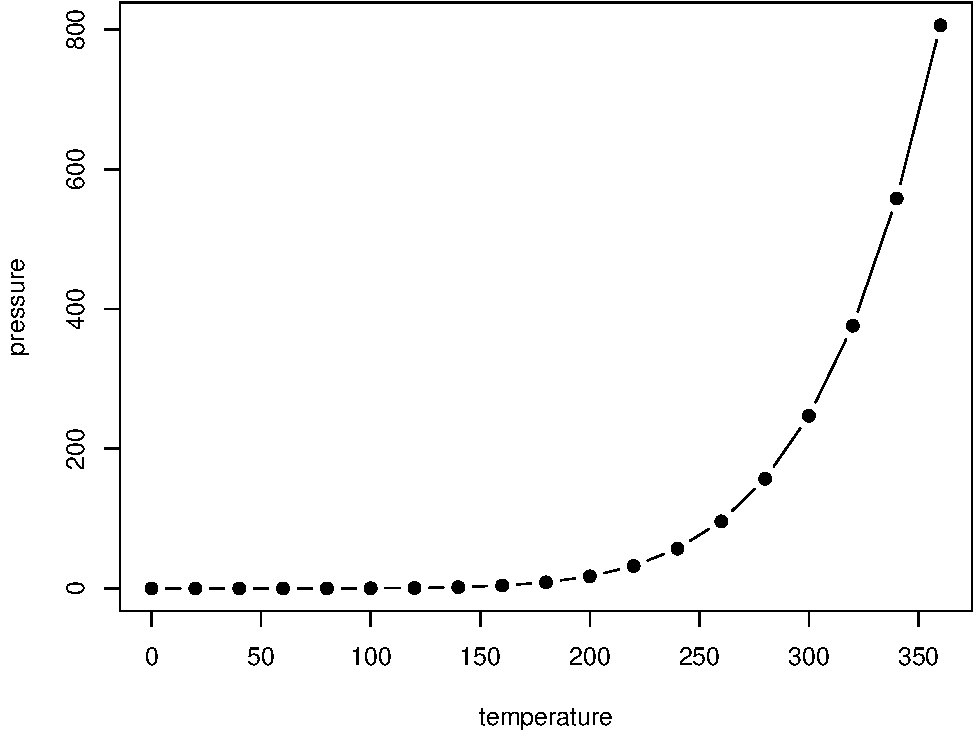
\includegraphics[width=0.8\linewidth]{AdvECTS_files/figure-latex/nice-fig-1} 

}

\caption{Here is a nice figure!}\label{fig:nice-fig}
\end{figure}

Reference a figure by its code chunk label with the \texttt{fig:} prefix, e.g., see Figure \ref{fig:nice-fig}. Similarly, you can reference tables generated from \texttt{knitr::kable()}, e.g., see Table \ref{tab:nice-tab}.

\begin{Shaded}
\begin{Highlighting}[]
\NormalTok{knitr}\SpecialCharTok{::}\FunctionTok{kable}\NormalTok{(}
  \FunctionTok{head}\NormalTok{(iris, }\DecValTok{20}\NormalTok{), }\AttributeTok{caption =} \StringTok{\textquotesingle{}Here is a nice table!\textquotesingle{}}\NormalTok{,}
  \AttributeTok{booktabs =} \ConstantTok{TRUE}
\NormalTok{)}
\end{Highlighting}
\end{Shaded}

\begin{table}

\caption{\label{tab:nice-tab}Here is a nice table!}
\centering
\begin{tabular}[t]{rrrrl}
\toprule
Sepal.Length & Sepal.Width & Petal.Length & Petal.Width & Species\\
\midrule
5.1 & 3.5 & 1.4 & 0.2 & setosa\\
4.9 & 3.0 & 1.4 & 0.2 & setosa\\
4.7 & 3.2 & 1.3 & 0.2 & setosa\\
4.6 & 3.1 & 1.5 & 0.2 & setosa\\
5.0 & 3.6 & 1.4 & 0.2 & setosa\\
\addlinespace
5.4 & 3.9 & 1.7 & 0.4 & setosa\\
4.6 & 3.4 & 1.4 & 0.3 & setosa\\
5.0 & 3.4 & 1.5 & 0.2 & setosa\\
4.4 & 2.9 & 1.4 & 0.2 & setosa\\
4.9 & 3.1 & 1.5 & 0.1 & setosa\\
\addlinespace
5.4 & 3.7 & 1.5 & 0.2 & setosa\\
4.8 & 3.4 & 1.6 & 0.2 & setosa\\
4.8 & 3.0 & 1.4 & 0.1 & setosa\\
4.3 & 3.0 & 1.1 & 0.1 & setosa\\
5.8 & 4.0 & 1.2 & 0.2 & setosa\\
\addlinespace
5.7 & 4.4 & 1.5 & 0.4 & setosa\\
5.4 & 3.9 & 1.3 & 0.4 & setosa\\
5.1 & 3.5 & 1.4 & 0.3 & setosa\\
5.7 & 3.8 & 1.7 & 0.3 & setosa\\
5.1 & 3.8 & 1.5 & 0.3 & setosa\\
\bottomrule
\end{tabular}
\end{table}

You can write citations, too. For example, we are using the \textbf{bookdown} package \citep{R-bookdown} in this sample book, which was built on top of R Markdown and \textbf{knitr} \citep{xie2015}.

Below is an example borrowed from \href{https://www.kellogg.northwestern.edu/faculty/petersen/htm/papers/se/test_data.htm}{Petersen}.

\begin{Shaded}
\begin{Highlighting}[]
\FunctionTok{library}\NormalTok{(sandwich)}
\DocumentationTok{\#\# Petersen\textquotesingle{}s data}
\FunctionTok{data}\NormalTok{(}\StringTok{"PetersenCL"}\NormalTok{, }\AttributeTok{package =} \StringTok{"sandwich"}\NormalTok{)}
\NormalTok{m }\OtherTok{\textless{}{-}} \FunctionTok{lm}\NormalTok{(y }\SpecialCharTok{\textasciitilde{}}\NormalTok{ x, }\AttributeTok{data =}\NormalTok{ PetersenCL)}

\DocumentationTok{\#\# clustered covariances}
\DocumentationTok{\#\# one{-}way}
\FunctionTok{vcovCL}\NormalTok{(m, }\AttributeTok{cluster =} \SpecialCharTok{\textasciitilde{}}\NormalTok{ firm)}
\end{Highlighting}
\end{Shaded}

\begin{verbatim}
##               (Intercept)             x
## (Intercept)  4.490702e-03 -6.473517e-05
## x           -6.473517e-05  2.559927e-03
\end{verbatim}

\begin{Shaded}
\begin{Highlighting}[]
\FunctionTok{vcovCL}\NormalTok{(m, }\AttributeTok{cluster =}\NormalTok{ PetersenCL}\SpecialCharTok{$}\NormalTok{firm) }\DocumentationTok{\#\# same}
\end{Highlighting}
\end{Shaded}

\begin{verbatim}
##               (Intercept)             x
## (Intercept)  4.490702e-03 -6.473517e-05
## x           -6.473517e-05  2.559927e-03
\end{verbatim}

\begin{Shaded}
\begin{Highlighting}[]
\DocumentationTok{\#\# one{-}way with HC2}
\FunctionTok{vcovCL}\NormalTok{(m, }\AttributeTok{cluster =} \SpecialCharTok{\textasciitilde{}}\NormalTok{ firm, }\AttributeTok{type =} \StringTok{"HC2"}\NormalTok{)}
\end{Highlighting}
\end{Shaded}

\begin{verbatim}
##               (Intercept)             x
## (Intercept)  4.494487e-03 -6.592912e-05
## x           -6.592912e-05  2.568236e-03
\end{verbatim}

\begin{Shaded}
\begin{Highlighting}[]
\DocumentationTok{\#\# two{-}way}
\FunctionTok{vcovCL}\NormalTok{(m, }\AttributeTok{cluster =} \SpecialCharTok{\textasciitilde{}}\NormalTok{ firm }\SpecialCharTok{+}\NormalTok{ year)}
\end{Highlighting}
\end{Shaded}

\begin{verbatim}
##               (Intercept)             x
## (Intercept)  4.233313e-03 -2.845344e-05
## x           -2.845344e-05  2.868462e-03
\end{verbatim}

\begin{Shaded}
\begin{Highlighting}[]
\FunctionTok{vcovCL}\NormalTok{(m, }\AttributeTok{cluster =}\NormalTok{ PetersenCL[, }\FunctionTok{c}\NormalTok{(}\StringTok{"firm"}\NormalTok{, }\StringTok{"year"}\NormalTok{)]) }\DocumentationTok{\#\# same}
\end{Highlighting}
\end{Shaded}

\begin{verbatim}
##               (Intercept)             x
## (Intercept)  4.233313e-03 -2.845344e-05
## x           -2.845344e-05  2.868462e-03
\end{verbatim}

XXXX

Sargan-Hansen () test. \citet{Sargan_1958} and \citet{Hansen_1982}

Durbin-Wu-Hausman test: \citet{Durbin_1954} / \citet{Wu_1973} / \citet{Hausman_1978}

\href{https://www.hds.utc.fr/~tdenoeux/dokuwiki/_media/en/kleibzeil_-_aer.pdf}{Use R!} is an excellent tutorial.
(notably for \texttt{plm} and the Arellano-Bond example, 140 UK firms)

Program evaluation (very good survey): \citet{Abadie_Cattaneo_2018}
Mostly harmless: \citet{angrist_mostly_2008}

Diff-in-Diff: \href{https://towardsdatascience.com/analyze-causal-effect-using-diff-in-diff-model-85e07b17e7b7}{Card and Krueger (1994)}

Diff-in-Diff:
\citet{Meyer_Viscusi_Durbin_1995}
with data in the \texttt{wooldridge} package. See \href{https://evalf20.classes.andrewheiss.com/example/diff-in-diff/}{this page}

\hypertarget{microeconometrics}{%
\chapter{Microeconometrics}\label{microeconometrics}}

\hypertarget{binary-choice-models}{%
\section{Binary-choice models}\label{binary-choice-models}}

In many instances, the variables to be explained (\(y_i\)s) have only two possible values (\(0\) and \(1\), say).

Assume we suspect some variable \(\mathbf{x}_i\) (\(K \times 1\)) to be able to account for the probability that \(y_i=1\).

The model reads:
\begin{equation}\label{eq:binaryBenroulli}
y_i | \mathbf{X} \sim \mathcal{B}(g(\mathbf{x}_i;\boldsymbol\theta)),
\end{equation}
where \(g(\mathbf{x}_i;\boldsymbol\theta)\) is the parameter of the Bernoulli distribution. In other words, conditionally on \(\mathbf{X}\):
\[
y_i = \left\{
\begin{array}{cl}
1 & \mbox{ with probability } g(\mathbf{x}_i;\boldsymbol\theta)\\
0 & \mbox{ with probability } 1-g(\mathbf{x}_i;\boldsymbol\theta),
\end{array}
\right.
\]
where \(\boldsymbol\theta\) is a vector of parameters to be estimated.

The objective is to estimate the vector of population parameters \(\boldsymbol\theta\).

Binary-choice models can be used to account for\ldots{}

\begin{itemize}
\tightlist
\item
  any binary decisions (e.g.~in referendums, being owner or renter, living in the city or in the countryside, in/out of the labour force,\ldots),
\item
  contamination (disease or default),
\item
  success/failure (exams).
\end{itemize}

A possibility is to run a linear regression (a situation called \textbf{Linear Probability Model, LPM}):
\[
y_i = \boldsymbol\theta'\mathbf{x}_i + \varepsilon_i.
\]

Such a regression could be consistent with the \emph{conditional-mean-zero assumption} (Hypothesis \ref{hyp:exogeneity}) and with the \emph{assumption of non-correlated residuals} (Hypothesis \ref{hyp:noncorrelResid}), but more difficultly with the \textbf{homoskedasticity assumption} (Hypothesis \ref{hyp:homoskedasticity}). Moreover, the \(\varepsilon_i\)s cannot be Gaussian (because \(y_i \in \{0,1\}\)). Therefore, using a linear regression to study the relationship between \(\mathbf{x}_i\) and \(y_i\) can be consistent but it is inefficient.

\begin{figure}

{\centering 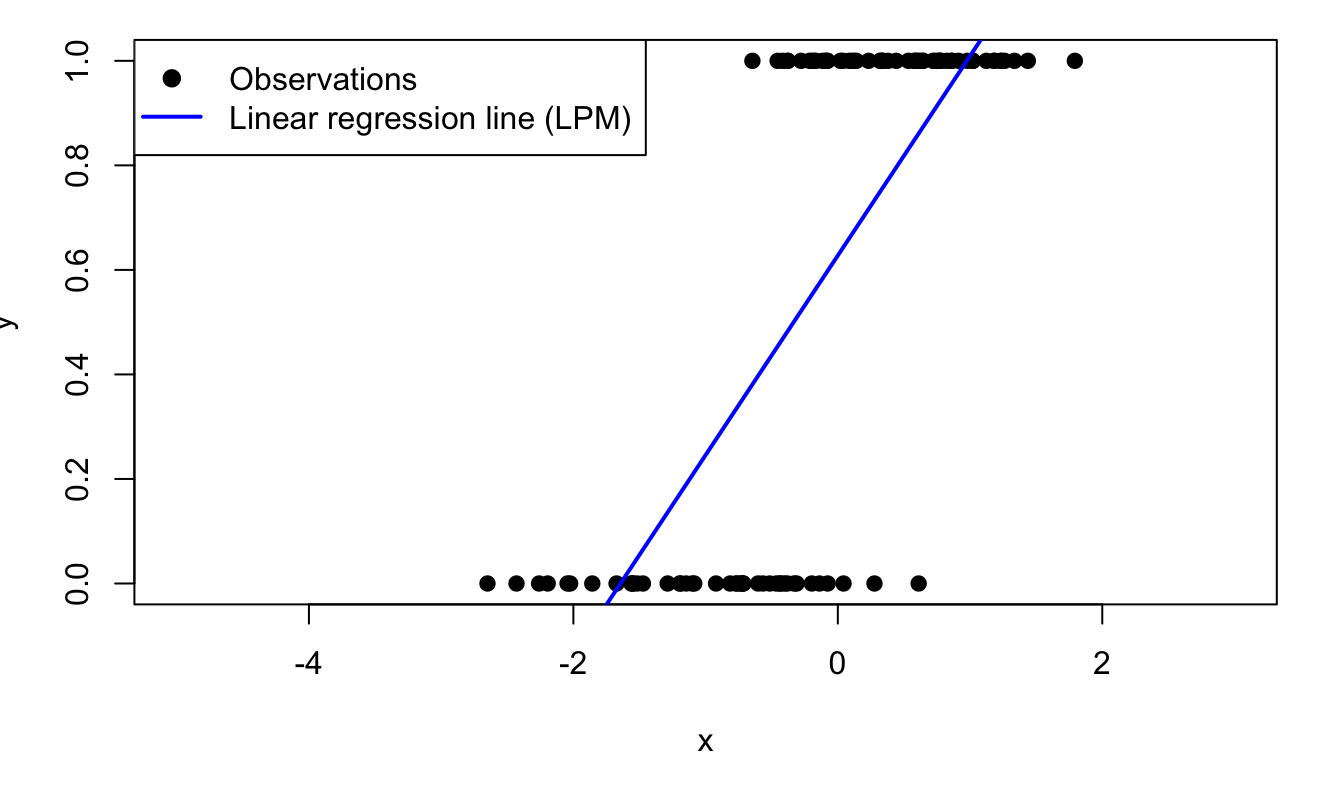
\includegraphics[width=0.9\linewidth]{AdvECTS_files/figure-latex/LPM-1} 

}

\caption{Fitting a binary variable with a linear model (Linear Probability Model, LPM). The model is $\mathbb{P}(y_i=1|x_i)=\Phi(0.5+2x_i)$, where $\Phi$ is the c.d.f. of the normal distribution and where $x_i \sim \,i.i.d.\,\mathcal{N}(0,1)$.}\label{fig:LPM}
\end{figure}

\begin{longtable}[]{@{}
  >{\raggedright\arraybackslash}p{(\columnwidth - 4\tabcolsep) * \real{0.0634}}
  >{\raggedright\arraybackslash}p{(\columnwidth - 4\tabcolsep) * \real{0.6972}}
  >{\raggedright\arraybackslash}p{(\columnwidth - 4\tabcolsep) * \real{0.2394}}@{}}
\caption{\label{tab:foo} This table provides examples of function \(g\), s.t. \(\mathbb{P}(y_i=1|\mathbf{x}_i;\boldsymbol heta) = g(\boldsymbol\theta'\mathbf{x}_i)\). The ``linear'' case is given for comparison, but note that it does not satisfy \(g(\boldsymbol\theta'\mathbf{x}_i)\) for any value of \(\boldsymbol\theta'\mathbf{x}_i\).}\tabularnewline
\toprule()
\begin{minipage}[b]{\linewidth}\raggedright
Model
\end{minipage} & \begin{minipage}[b]{\linewidth}\raggedright
Function \(g\)
\end{minipage} & \begin{minipage}[b]{\linewidth}\raggedright
Derivative
\end{minipage} \\
\midrule()
\endfirsthead
\toprule()
\begin{minipage}[b]{\linewidth}\raggedright
Model
\end{minipage} & \begin{minipage}[b]{\linewidth}\raggedright
Function \(g\)
\end{minipage} & \begin{minipage}[b]{\linewidth}\raggedright
Derivative
\end{minipage} \\
\midrule()
\endhead
Probit & \(\Phi\) & \(\phi\) \\
Logit & \(\dfrac{\exp(x)}{1+\exp(x)}\) & \(\dfrac{\exp(x)}{(1+\exp(x))^2}\) \\
log-log & \(1 - \exp(-\exp(x))\) & \(\exp(-\exp(x))\exp(x)\) \\
linear & \(x\) & 1 \\
\bottomrule()
\end{longtable}

Two prominent models to tackle this situation. In both models, we have:
\[
\mathbb{P}(y_i=1|\mathbf{x}_i;\boldsymbol\theta)=g(\boldsymbol\theta'\mathbf{x}_i).
\]

In the \textbf{Probit model}, we have
\begin{equation}
g(z) = \Phi(z),\label{eq:probit}
\end{equation}
where \(\Phi\) is the c.d.f. of the normal distribution.

And for the \textbf{logit model}:
\begin{equation}
g(z) = \frac{1}{1+\exp(-z)}.\label{eq:logit}
\end{equation}

Figure \ref{fig:ProbLogit} displays the functions \(g\) appearing in Table \ref{tab:foo}.

\begin{figure}

{\centering 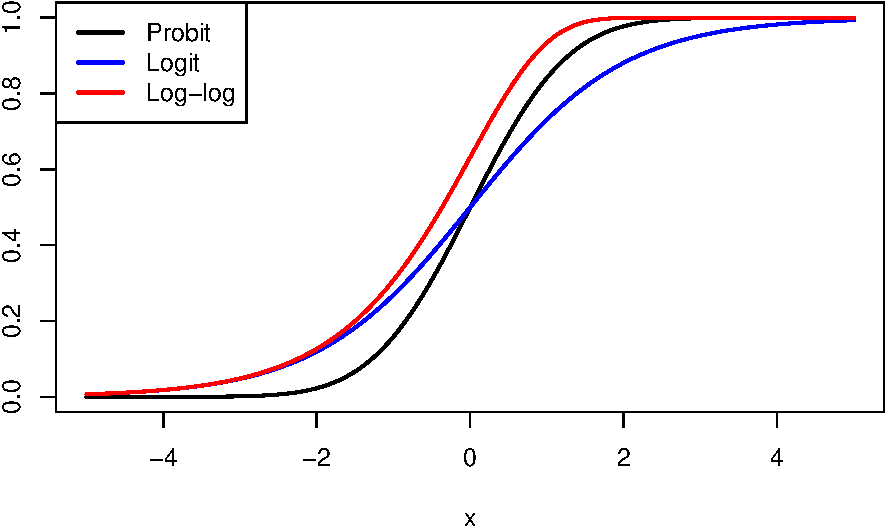
\includegraphics[width=0.9\linewidth]{AdvECTS_files/figure-latex/ProbLogit-1} 

}

\caption{Probit, Logit, and Log-log functions.}\label{fig:ProbLogit}
\end{figure}

\begin{figure}

{\centering 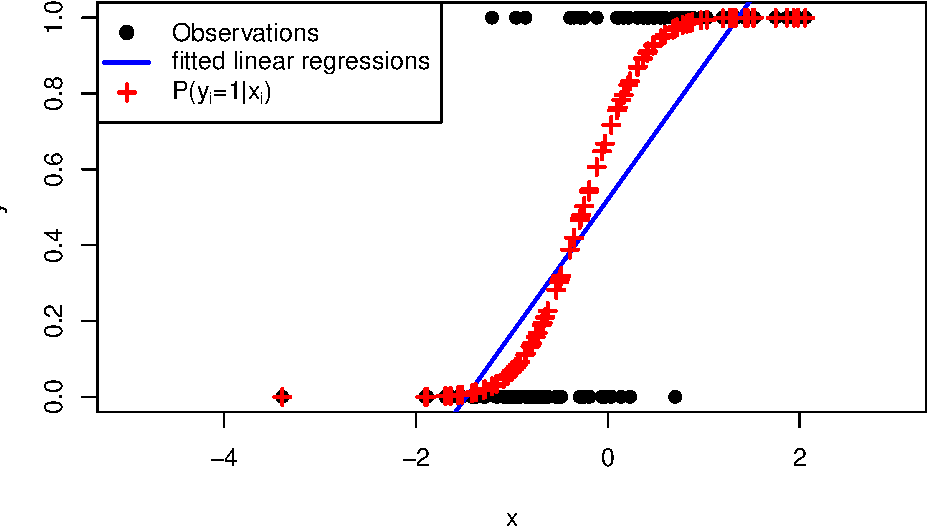
\includegraphics[width=0.9\linewidth]{AdvECTS_files/figure-latex/LPM2-1} 

}

\caption{The model is $\mathbb{P}(y_i=1|x_i)=\Phi(0.5+2x_i)$, where $\Phi$ is the c.d.f. of the normal distribution and where $x_i \sim \,i.i.d.\,\mathcal{N}(0,1)$. Crosses give the model-implied probabilities of having $y_i=1$.}\label{fig:LPM2}
\end{figure}

\hypertarget{interpretation-in-terms-of-latent-variable-and-utility-based-models}{%
\subsection{Interpretation in terms of latent variable, and utility-based models}\label{interpretation-in-terms-of-latent-variable-and-utility-based-models}}

The probit model has an interpretation in terms of \textbf{latent variables}. In this model, we indeed have:
\[
\mathbb{P}(y_i=1|\mathbf{x}_i;\boldsymbol\theta) = \Phi(\boldsymbol\theta'\mathbf{x}_i) = \mathbb{P}(-\varepsilon_{i}<\boldsymbol\theta'\mathbf{x}_i),
\]
where \(\varepsilon_{i} \sim \mathcal{N}(0,1)\). That is:
\[
\mathbb{P}(y_i=1|\mathbf{x}_i;\boldsymbol\theta) = \mathbb{P}(0< y_i^*),
\]
where \(y_i^* = \boldsymbol\theta'\mathbf{x}_i + \varepsilon_i\), with \(\varepsilon_{i} \sim \mathcal{N}(0,1)\). Variable \(y_i^*\) can be interpreted as a (latent) variable that determines \(y_i\) since \(y_i = \mathbb{I}_{\{y_i^*>0\}}\).

\begin{figure}

{\centering 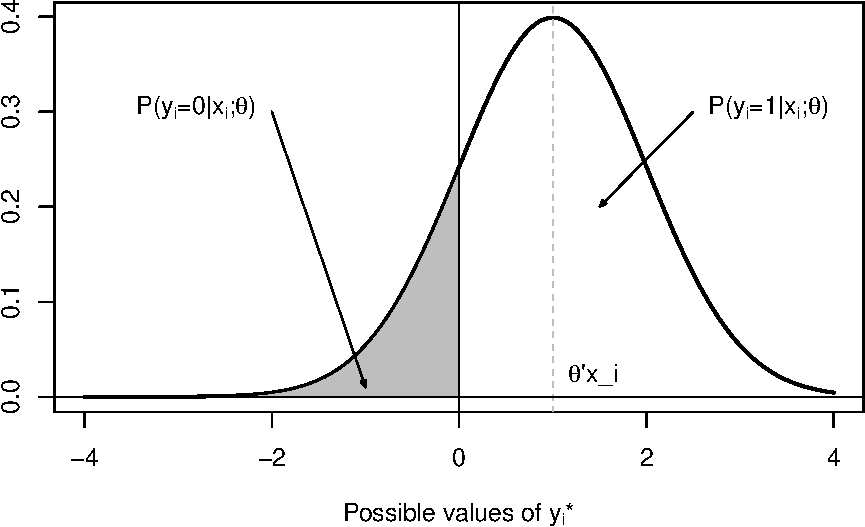
\includegraphics[width=0.9\linewidth]{AdvECTS_files/figure-latex/Latent-1} 

}

\caption{Distribution of $y_i^*$ conditional on $\mathbf{x}_i$.}\label{fig:Latent}
\end{figure}

\textbf{Random Utility Models (RUM)} are based on such a view of probit models. Assume that agent (\(i\)) chooses \(y_i=1\) if the utility associated with this choice (\(U_{i,1}\)) is higher than the one associated with \(y_i=0\) (\(U_{i,0}\)). Assume further that the utility of agent \(i\), if she chooses outcome \(j\) (\(\in \{0,1\}\)), is given by
\[
U_{i,j} = V_{i,j} + \varepsilon_{i,j},
\]
where \(V_{i,j}\) is the deterministic component of the utility associated with choice and \(\varepsilon_{i,j}\) is a random (agent-specific) component.

Moreover, posit \(V_{i,j} = \boldsymbol\theta_j'\mathbf{x}_i\). We then have:
\begin{eqnarray}
\mathbb{P}(y_i = 1|\mathbf{x}_i;\boldsymbol\theta) &=& \mathbb{P}(\boldsymbol\theta_1'\mathbf{x}_i+\varepsilon_{i,1}>\boldsymbol\theta_0'\mathbf{x}_i+\varepsilon_{i,0}) \nonumber\\
&=& F(\boldsymbol\theta_1'\mathbf{x}_i-\boldsymbol\theta_0'\mathbf{x}_i) = F([\boldsymbol\theta_1-\boldsymbol\theta_0]'\mathbf{x}_i),\label{eq:utility}
\end{eqnarray}
where \(F\) is the c.d.f. of \(\varepsilon_{i,0}-\varepsilon_{i,1}\).

Note that only the difference \(\boldsymbol\theta_1-\boldsymbol\theta_0\) is identifiable (as opposed to \(\boldsymbol\theta_1\) AND \(\boldsymbol\theta_0\)). Indeed, replacing \(U\) with \(aU\) (\(a>0\)) gives the same model \(\Leftrightarrow\) scaling issue, solved by fixing the variance of \(\varepsilon_{i,0}-\varepsilon_{i,1}\).

Other types of structural models --based on the comparison of marginal costs and benefits-- give rise to the existence of latent variable and to probit models. An example is \citet{Nakosteen_Zimmer_1980}. The main ingredients of their approach are as follows:

\begin{itemize}
\item
  Wage that can be earned at the present location: \(y_p^* = \boldsymbol\theta_p'\mathbf{x}_p + \varepsilon_p\).
\item
  Migration cost: \(C^*= \boldsymbol\theta_c'\mathbf{x}_c + \varepsilon_c\).
\item
  Wage earned elsewhere: \(y_m^* = \boldsymbol\theta_m'\mathbf{x}_m + \varepsilon_m\).
\end{itemize}

In this context, agents decision to migrate if \(y_m^* > y_p^* + C^*\), i.e.~if
\[
y^* = y_m^* -  y_p^* - C^* =  \boldsymbol\theta'\mathbf{x} + \underbrace{\varepsilon}_{=\varepsilon_m - \varepsilon_c - \varepsilon_p}>0,
\]
where \(\mathbf{x}\) is the union of the \(\mathbf{x}_i\)s, for \(i \in \{p,m,c\}\).

\hypertarget{Avregressors}{%
\subsection{Alternative-Varying Regressors}\label{Avregressors}}

In some cases, the regressors may depend on the considered alternative (\(0\) or \(1\)). For instance:

\begin{itemize}
\item
  When modeling the decision to participate in the labour force (or not), the wage depends on the alternative. It cannot be included among the regressors given it is not observed if the considered agent has decided not to work.
\item
  In the context of the choice of transportation mode, the \emph{time cost} depends on the considered transportation mode.
\end{itemize}

In terms of utility, we then have:
\[
V_{i,j} = {\theta^{(u)}_{j}}'\mathbf{u}_{i,j} + {\theta^{(v)}_{j}}'\mathbf{v}_{i},
\]
where the \(\mathbf{u}_{i,j}\)s are regressors associated with agent \(i\), but taking different values for the different choices (\(j=0\) or \(j=1\)).

In that case, Eq. \eqref{eq:utility} becomes:
\begin{equation}
\mathbb{P}(y_i = 1|\mathbf{x}_i;\boldsymbol\theta)  = F\left({\theta^{(u)}_{1}}'\mathbf{u}_{i,1}-{\theta^{(u)}_{0}}'\mathbf{u}_{i,0}+[\boldsymbol\theta_1^{(v)}-\boldsymbol\theta_0^{(v)}]'\mathbf{v}_i\right),\label{eq:utility2}
\end{equation}
and, if \(\theta^{(u)}_{1}=\theta^{(u)}_{0}=\theta^{(u)}\) --as is customary-- we get:
\begin{equation}
\mathbb{P}(y_i = 1|\mathbf{x}_i;\boldsymbol\theta)  = F\left({\theta^{(u)}_{1}}'(\mathbf{u}_{i,1}-\mathbf{u}_{i,0})+[\boldsymbol\theta_1^{(v)}-\boldsymbol\theta_0^{(v)}]'\mathbf{v}_i\right).\label{eq:utility3}
\end{equation}

The fishing-mode dataset used in \citet{Cameron_Trivedi_2005} (Chapter 14 and 15) contains alternative-specific variables. Specifically, for each individual, the price and catch rate depend on the fishing model. In the table reported below, lines \texttt{price} and \texttt{catch} correspond to the prices and catch rates associated with the chosen alternative.

\begin{Shaded}
\begin{Highlighting}[]
\FunctionTok{library}\NormalTok{(Ecdat)}
\FunctionTok{data}\NormalTok{(Fishing)}
\NormalTok{stargazer}\SpecialCharTok{::}\FunctionTok{stargazer}\NormalTok{(Fishing,}\AttributeTok{type=}\StringTok{"text"}\NormalTok{)}
\end{Highlighting}
\end{Shaded}

\begin{verbatim}
## 
## ======================================================
## Statistic   N     Mean    St. Dev.    Min      Max    
## ------------------------------------------------------
## price     1,182  52.082    53.830    1.290   666.110  
## catch     1,182   0.389     0.561   0.0002    2.310   
## pbeach    1,182  103.422   103.641   1.290   843.186  
## ppier     1,182  103.422   103.641   1.290   843.186  
## pboat     1,182  55.257    62.713    2.290   666.110  
## pcharter  1,182  84.379    63.545   27.290   691.110  
## cbeach    1,182   0.241     0.191    0.068    0.533   
## cpier     1,182   0.162     0.160    0.001    0.452   
## cboat     1,182   0.171     0.210   0.0002    0.737   
## ccharter  1,182   0.629     0.706    0.002    2.310   
## income    1,182 4,099.337 2,461.964 416.667 12,500.000
## ------------------------------------------------------
\end{verbatim}

\hypertarget{estimation}{%
\subsection{Estimation}\label{estimation}}

These models can be estimated by Maximum Likelihood approaches (see Section \ref{secMLE}).

To simplify the exposition, we consider the \(\mathbf{x}_i\) to be deterministic. Also, we assume that the r.v. are independent across entities \(i\). How to write the likelihood here? It can be seen that:
\begin{eqnarray}
f(y_i|\mathbf{x}_i;\boldsymbol\theta) &=& y_i g(\boldsymbol\theta'\mathbf{x}_i) + (1-y_i) (1-g(\boldsymbol\theta'\mathbf{x}_i)) \nonumber \\
&=&  g(\boldsymbol\theta'\mathbf{x}_i)^{y_i}(1-g(\boldsymbol\theta'\mathbf{x}_i))^{1-y_i}.
\end{eqnarray}

Therefore, if the observations \((\mathbf{x}_i,y_i)\) are independent across entities \(i\), then:
\[
\log \mathcal{L}(\boldsymbol\theta;\mathbf{y},\mathbf{X}) = \sum_{i=1}^{n}y_i \log[g(\boldsymbol\theta'\mathbf{x}_i)] + (1-y_i)\log[1-g(\boldsymbol\theta'\mathbf{x}_i)].
\]

The likelihood equation reads (FOC of the optimization program, see Def. \ref{def:likFunction}):
\[
\dfrac{\partial \log \mathcal{L}(\boldsymbol\theta;\mathbf{y},\mathbf{X})}{\partial \boldsymbol\theta} = \mathbf{0},
\]
that is:
\[
\sum_{i=1}^{n} y_i \mathbf{x}_i\frac{g'(\boldsymbol\theta'\mathbf{x}_i)}{g(\boldsymbol\theta'\mathbf{x}_i)} - (1-y_i) \mathbf{x}_i \frac{g'(\boldsymbol\theta'\mathbf{x}_i)}{1-g(\boldsymbol\theta'\mathbf{x}_i)} = \mathbf{0}.
\]

This is a nonlinear equation that generally has to be numerically solved. Under regularity conditions (Hypotheses \ref{hyp:MLEregularity}), we have (Prop. \ref{prp:MLEproperties}):
\[
\boldsymbol\theta_{MLE} \sim \mathcal{N}(\boldsymbol\theta_0,\mathbf{I}(\boldsymbol\theta_0)^{-1}),
\]
where
\[
\mathbf{I}(\boldsymbol\theta_0) = - \mathbb{E}_0 \left( \frac{\partial^2 \log \mathcal{L}(\theta;\mathbf{y},\mathbf{X})}{\partial \boldsymbol\theta \partial \boldsymbol\theta'}\right) = n \mathcal{I}_Y(\boldsymbol\theta_0).
\]

For finite samples, we can e.g.~approximate \(\mathbf{I}(\boldsymbol\theta_0)^{-1}\) by (Eq. \eqref{eq:III1}):
\[
\mathbf{I}(\boldsymbol\theta_0)^{-1} \approx -\left(\frac{\partial^2 \log \mathcal{L}(\boldsymbol\theta_{MLE};\mathbf{y},\mathbf{X})}{\partial \boldsymbol\theta \partial \boldsymbol\theta'}\right)^{-1}.
\]

In the Probit case (see Table \ref{tab:foo}), it can be shown that we have:
\begin{eqnarray*}
&&\frac{\partial^2 \log \mathcal{L}(\boldsymbol\theta;\mathbf{y},\mathbf{X})}{\partial \boldsymbol\theta \partial \boldsymbol\theta'} = - \sum_{i=1}^{n} g'(\boldsymbol\theta'\mathbf{x}_i) [\mathbf{x}_i \mathbf{x}_i'] \times \\
&&\left[y_i \frac{g'(\boldsymbol\theta'\mathbf{x}_i) + \boldsymbol\theta'\mathbf{x}_ig(\boldsymbol\theta'\mathbf{x}_i)}{g(\boldsymbol\theta'\mathbf{x}_i)^2} + (1-y_i) \frac{g'(\boldsymbol\theta'\mathbf{x}_i) - \boldsymbol\theta'\mathbf{x}_i (1 - g(\boldsymbol\theta'\mathbf{x}_i))}{(1-g(\boldsymbol\theta'\mathbf{x}_i))^2}\right].
\end{eqnarray*}

In the Logit case (see Table \ref{tab:foo}), it can be shown that we have:
\[
\frac{\partial^2 \log \mathcal{L}(\boldsymbol\theta;\mathbf{y},\mathbf{X})}{\partial \boldsymbol\theta \partial \boldsymbol\theta'} = - \sum_{i=1}^{n} g'(\boldsymbol\theta'\mathbf{x}_i) \mathbf{x}_i\mathbf{x}_i',
\]
where \(g'(x)=\dfrac{\exp(-x)}{(1 + \exp(-x))^2}\).

Since \(g'(x)>0\), it can be checked that \(-\partial^2 \log \mathcal{L}(\boldsymbol\theta;\mathbf{y},\mathbf{X})/\partial \boldsymbol\theta \partial \boldsymbol\theta'\) is positive definite.

\hypertarget{marginal-effectss}{%
\subsection{Marginal effectss}\label{marginal-effectss}}

How to measure marginal effects, i.e.~the effect on the probability that \(y_i=1\) of a marginal increase of \(x_{i,k}\)? This object is given by:
\[
\frac{\partial \mathbb{P}(y_i=1|\mathbf{x_i};\boldsymbol\theta)}{\partial x_{i,k}} = \underbrace{g'(\boldsymbol\theta'\mathbf{x}_i)}_{>0}\theta_k,
\]
which is of the same sign as \(\theta_k\).

It can be estimated by \(g'(\boldsymbol\theta_{MLE}'\mathbf{x}_i)\theta_{MLE,k}\). It is important to see that the marginal effect depends on \(\mathbf{x}_i\): increases by 1 unit of \(x_{i,k}\) (entity \(i\)) and of \(x_{j,k}\) (entity \(j\)) do not necessarily have the same effects on \(\mathbb{P}(y_i=1|\mathbf{x_i};\boldsymbol\theta)\) and on \(\mathbb{P}(y_j=1|\mathbf{x_j};\boldsymbol\theta)\), respectively.

To address this issue, one can compute some measures of ``average'' marginal effect. There are two main solutions. For each explanatory variable \(k\):

\begin{enumerate}
\def\labelenumi{\roman{enumi}.}
\item
  Denoting by \(\hat{\mathbf{x}}\) the sample average of the \(\mathbf{x}_i\)s, compute \(g'(\boldsymbol\theta_{MLE}'\hat{\mathbf{x}})\theta_{MLE,k}\).
\item
  Compute the average (across \(i\)) of \(g'(\boldsymbol\theta_{MLE}'\mathbf{x}_i)\theta_{MLE,k}\).
\end{enumerate}

\hypertarget{goodness-of-fit}{%
\subsection{Goodness of fit}\label{goodness-of-fit}}

There is no obvious version of ``\(R^2\)'' for binary-choice models. Existing measures are called \textbf{pseudo-\(R^2\)\} measures}.

Denoting by \(\log \mathcal{L}_0(\mathbf{y})\) the (maximum) log-likelihood that would be obtained for a model containing only a constant term (i.e.~with \(\mathbf{x}_i = 1\) for all \(i\)), the \textbf{McFadden's pseudo-\(R^2\)} is given by:
\[
R^2_{MF} = 1 - \frac{\log \mathcal{L}(\boldsymbol\theta;\mathbf{y})}{\log \mathcal{L}_0(\mathbf{y})}.
\]
Intuitively, \(R^2_{MF}=0\) if the explanatory variables do not allow to predict the decision (\(y\)).

\hypertarget{example-credit-data}{%
\subsection{Example: Credit data}\label{example-credit-data}}

This example makes use of the \texttt{credit} data of package \texttt{AEC}. The objective is to model the default probabilities of lenders.

\begin{Shaded}
\begin{Highlighting}[]
\FunctionTok{library}\NormalTok{(AEC)}
\NormalTok{credit}\SpecialCharTok{$}\NormalTok{Default }\OtherTok{\textless{}{-}} \DecValTok{0}
\NormalTok{credit}\SpecialCharTok{$}\NormalTok{Default[credit}\SpecialCharTok{$}\NormalTok{loan\_status }\SpecialCharTok{==} \StringTok{"Charged Off"}\NormalTok{] }\OtherTok{\textless{}{-}} \DecValTok{1}
\NormalTok{credit}\SpecialCharTok{$}\NormalTok{Default[credit}\SpecialCharTok{$}\NormalTok{loan\_status }\SpecialCharTok{==} \StringTok{"Does not meet the credit policy. Status:Charged Off"}\NormalTok{] }\OtherTok{\textless{}{-}} \DecValTok{1}
\NormalTok{credit}\SpecialCharTok{$}\NormalTok{amt2income }\OtherTok{\textless{}{-}}\NormalTok{ credit}\SpecialCharTok{$}\NormalTok{loan\_amnt}\SpecialCharTok{/}\NormalTok{credit}\SpecialCharTok{$}\NormalTok{annual\_inc}
\FunctionTok{plot}\NormalTok{(}\FunctionTok{as.factor}\NormalTok{(credit}\SpecialCharTok{$}\NormalTok{Default)}\SpecialCharTok{\textasciitilde{}}\FunctionTok{log}\NormalTok{(credit}\SpecialCharTok{$}\NormalTok{annual\_inc),}
     \AttributeTok{ylevels=}\DecValTok{2}\SpecialCharTok{:}\DecValTok{1}\NormalTok{,}\AttributeTok{ylab=}\StringTok{"Default status"}\NormalTok{,}\AttributeTok{xlab=}\StringTok{"log(annual income)"}\NormalTok{)}
\end{Highlighting}
\end{Shaded}

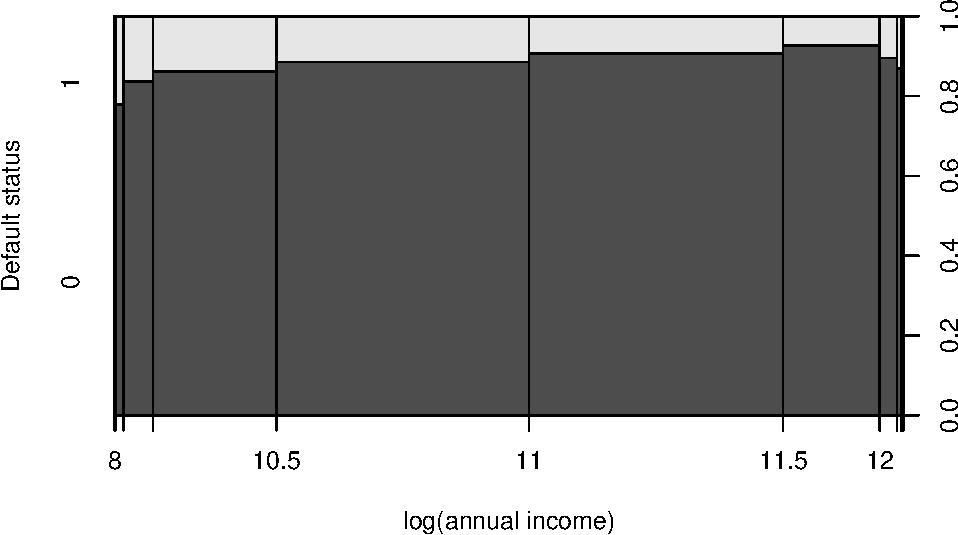
\includegraphics{AdvECTS_files/figure-latex/Probitlending-1.pdf}

We consider three specifications. The first one, with no explanatory variables, is trivial. It will just be used to compute the pseudo-\(R^2\).

\begin{Shaded}
\begin{Highlighting}[]
\NormalTok{eq0 }\OtherTok{\textless{}{-}} \FunctionTok{glm}\NormalTok{(Default }\SpecialCharTok{\textasciitilde{}} \DecValTok{1}\NormalTok{,}\AttributeTok{data=}\NormalTok{credit,}\AttributeTok{family=}\FunctionTok{binomial}\NormalTok{(}\AttributeTok{link=}\StringTok{"probit"}\NormalTok{))}
\NormalTok{eq1 }\OtherTok{\textless{}{-}} \FunctionTok{glm}\NormalTok{(Default }\SpecialCharTok{\textasciitilde{}} \FunctionTok{log}\NormalTok{(loan\_amnt) }\SpecialCharTok{+}\NormalTok{ amt2income }\SpecialCharTok{+}\NormalTok{ delinq\_2yrs }\SpecialCharTok{+} \FunctionTok{log}\NormalTok{(annual\_inc)}\SpecialCharTok{+} \FunctionTok{I}\NormalTok{(}\FunctionTok{log}\NormalTok{(annual\_inc)}\SpecialCharTok{\^{}}\DecValTok{2}\NormalTok{),}
                 \AttributeTok{data=}\NormalTok{credit,}\AttributeTok{family=}\FunctionTok{binomial}\NormalTok{(}\AttributeTok{link=}\StringTok{"probit"}\NormalTok{))}
\NormalTok{eq2 }\OtherTok{\textless{}{-}} \FunctionTok{glm}\NormalTok{(Default }\SpecialCharTok{\textasciitilde{}}\NormalTok{ grade }\SpecialCharTok{+} \FunctionTok{log}\NormalTok{(loan\_amnt) }\SpecialCharTok{+}\NormalTok{ amt2income }\SpecialCharTok{+}\NormalTok{ delinq\_2yrs }\SpecialCharTok{+} \FunctionTok{log}\NormalTok{(annual\_inc)}\SpecialCharTok{+} \FunctionTok{I}\NormalTok{(}\FunctionTok{log}\NormalTok{(annual\_inc)}\SpecialCharTok{\^{}}\DecValTok{2}\NormalTok{),}
                 \AttributeTok{data=}\NormalTok{credit,}\AttributeTok{family=}\FunctionTok{binomial}\NormalTok{(}\AttributeTok{link=}\StringTok{"probit"}\NormalTok{))}
\NormalTok{logL0 }\OtherTok{\textless{}{-}} \FunctionTok{logLik}\NormalTok{(eq0)}
\NormalTok{logL1 }\OtherTok{\textless{}{-}} \FunctionTok{logLik}\NormalTok{(eq1)}
\NormalTok{logL2 }\OtherTok{\textless{}{-}} \FunctionTok{logLik}\NormalTok{(eq2)}
\DecValTok{1} \SpecialCharTok{{-}}\NormalTok{ logL1}\SpecialCharTok{/}\NormalTok{logL0 }\CommentTok{\# pseudo R2}
\end{Highlighting}
\end{Shaded}

\begin{verbatim}
## 'log Lik.' 0.01173993 (df=6)
\end{verbatim}

\begin{Shaded}
\begin{Highlighting}[]
\DecValTok{1} \SpecialCharTok{{-}}\NormalTok{ logL2}\SpecialCharTok{/}\NormalTok{logL0 }\CommentTok{\# pseudo R2}
\end{Highlighting}
\end{Shaded}

\begin{verbatim}
## 'log Lik.' 0.0558487 (df=12)
\end{verbatim}

\begin{Shaded}
\begin{Highlighting}[]
\NormalTok{stargazer}\SpecialCharTok{::}\FunctionTok{stargazer}\NormalTok{(eq0,eq1,eq2,}\AttributeTok{type=}\StringTok{"text"}\NormalTok{)}
\end{Highlighting}
\end{Shaded}

\begin{verbatim}
## 
## ====================================================
##                           Dependent variable:       
##                     --------------------------------
##                                 Default             
##                        (1)        (2)        (3)    
## ----------------------------------------------------
## gradeB                                     0.400*** 
##                                            (0.055)  
##                                                     
## gradeC                                     0.587*** 
##                                            (0.057)  
##                                                     
## gradeD                                     0.820*** 
##                                            (0.061)  
##                                                     
## gradeE                                     0.874*** 
##                                            (0.091)  
##                                                     
## gradeF                                     1.230*** 
##                                            (0.147)  
##                                                     
## gradeG                                     1.439*** 
##                                            (0.227)  
##                                                     
## log(loan_amnt)                  -0.149**  -0.194*** 
##                                 (0.060)    (0.061)  
##                                                     
## amt2income                      1.266***   1.222*** 
##                                 (0.383)    (0.393)  
##                                                     
## delinq_2yrs                     0.096***    0.009   
##                                 (0.034)    (0.035)  
##                                                     
## log(annual_inc)                 -1.444**    -0.874  
##                                 (0.569)    (0.586)  
##                                                     
## I(log(annual_inc)2)             0.064**     0.038   
##                                 (0.025)    (0.026)  
##                                                     
## Constant            -1.231***   7.937***    4.749   
##                      (0.017)    (3.060)    (3.154)  
##                                                     
## ----------------------------------------------------
## Observations          9,156      9,156      9,156   
## Log Likelihood      -3,157.696 -3,120.625 -2,981.343
## Akaike Inf. Crit.   6,317.392  6,253.250  5,986.686 
## ====================================================
## Note:                    *p<0.1; **p<0.05; ***p<0.01
\end{verbatim}

Let us now compute marginal effects.

\begin{Shaded}
\begin{Highlighting}[]
\FunctionTok{mean}\NormalTok{(}\FunctionTok{dnorm}\NormalTok{(}\FunctionTok{predict}\NormalTok{(eq2)),}\AttributeTok{na.rm=}\ConstantTok{TRUE}\NormalTok{)}\SpecialCharTok{*}\NormalTok{eq2}\SpecialCharTok{$}\NormalTok{coefficients}
\end{Highlighting}
\end{Shaded}

\begin{verbatim}
##          (Intercept)               gradeB               gradeC 
##          0.840731198          0.070747353          0.103944305 
##               gradeD               gradeE               gradeF 
##          0.145089219          0.154773742          0.217702041 
##               gradeG       log(loan_amnt)           amt2income 
##          0.254722161         -0.034289921          0.216251992 
##          delinq_2yrs      log(annual_inc) I(log(annual_inc)^2) 
##          0.001574178         -0.154701321          0.006813694
\end{verbatim}

There is, however, an issue for the \texttt{annual\_inc} variable. Indeed, the previous computation does not realize that this variable appears twice among the explanatory variables. To address this, one can proceed as follows.

\begin{Shaded}
\begin{Highlighting}[]
\NormalTok{new\_credit }\OtherTok{\textless{}{-}}\NormalTok{ credit}
\NormalTok{new\_credit}\SpecialCharTok{$}\NormalTok{annual\_inc }\OtherTok{\textless{}{-}} \FloatTok{1.01} \SpecialCharTok{*}\NormalTok{ new\_credit}\SpecialCharTok{$}\NormalTok{annual\_inc }\CommentTok{\# increase of income by 1\%}
\NormalTok{bas\_predict\_eq2  }\OtherTok{\textless{}{-}} \FunctionTok{predict}\NormalTok{(eq2, }\AttributeTok{newdata =}\NormalTok{ credit, }\AttributeTok{type =} \StringTok{"response"}\NormalTok{)}
\CommentTok{\# This is equivalent to pnorm(predict(eq2, newdata = credit))}
\NormalTok{new\_predict\_eq2  }\OtherTok{\textless{}{-}} \FunctionTok{predict}\NormalTok{(eq2, }\AttributeTok{newdata =}\NormalTok{ new\_credit, }\AttributeTok{type =} \StringTok{"response"}\NormalTok{)}
\FunctionTok{mean}\NormalTok{(new\_predict\_eq2 }\SpecialCharTok{{-}}\NormalTok{ bas\_predict\_eq2)}
\end{Highlighting}
\end{Shaded}

\begin{verbatim}
## [1] -6.562126e-05
\end{verbatim}

This average effect is pretty low. To compare, let us compute the average effect associated with a unit increase in the number of delinquencies:

\begin{Shaded}
\begin{Highlighting}[]
\NormalTok{new\_credit }\OtherTok{\textless{}{-}}\NormalTok{ credit}
\NormalTok{new\_credit}\SpecialCharTok{$}\NormalTok{delinq\_2yrs }\OtherTok{\textless{}{-}}\NormalTok{ credit}\SpecialCharTok{$}\NormalTok{delinq\_2yrs }\SpecialCharTok{+} \DecValTok{1}
\NormalTok{new\_predict\_eq2  }\OtherTok{\textless{}{-}} \FunctionTok{predict}\NormalTok{(eq2, }\AttributeTok{newdata =}\NormalTok{ new\_credit, }\AttributeTok{type =} \StringTok{"response"}\NormalTok{)}
\FunctionTok{mean}\NormalTok{(new\_predict\_eq2 }\SpecialCharTok{{-}}\NormalTok{ bas\_predict\_eq2)}
\end{Highlighting}
\end{Shaded}

\begin{verbatim}
## [1] 0.001582332
\end{verbatim}

We can employ a likelihood ratio test (see Def. \ref{def:LR}) to see if the two variables associated with annual income are jointly statistically significant (in the context of \texttt{eq1}):

\begin{Shaded}
\begin{Highlighting}[]
\NormalTok{eq1restr }\OtherTok{\textless{}{-}} \FunctionTok{glm}\NormalTok{(Default }\SpecialCharTok{\textasciitilde{}} \FunctionTok{log}\NormalTok{(loan\_amnt) }\SpecialCharTok{+}\NormalTok{ amt2income }\SpecialCharTok{+}\NormalTok{ delinq\_2yrs,}
                 \AttributeTok{data=}\NormalTok{credit,}\AttributeTok{family=}\FunctionTok{binomial}\NormalTok{(}\AttributeTok{link=}\StringTok{"probit"}\NormalTok{))}
\NormalTok{LRstat }\OtherTok{\textless{}{-}} \DecValTok{2}\SpecialCharTok{*}\NormalTok{(logL1 }\SpecialCharTok{{-}} \FunctionTok{logLik}\NormalTok{(eq1restr))}
\NormalTok{pvalue }\OtherTok{\textless{}{-}} \DecValTok{1} \SpecialCharTok{{-}} \FunctionTok{c}\NormalTok{(}\FunctionTok{pchisq}\NormalTok{(LRstat,}\AttributeTok{df=}\DecValTok{2}\NormalTok{))}
\end{Highlighting}
\end{Shaded}

The computation gives a p-value of 0.0436.

\hypertarget{replicating-table-14.2-of-cameron-and-trivedi-2005}{%
\subsection{Replicating Table 14.2 of Cameron and Trivedi (2005)}\label{replicating-table-14.2-of-cameron-and-trivedi-2005}}

The following lines of codes replicate Table 14.2 of \citet{Cameron_Trivedi_2005}.

\begin{Shaded}
\begin{Highlighting}[]
\NormalTok{data.reduced }\OtherTok{\textless{}{-}} \FunctionTok{subset}\NormalTok{(Fishing,mode }\SpecialCharTok{\%in\%} \FunctionTok{c}\NormalTok{(}\StringTok{"charter"}\NormalTok{,}\StringTok{"pier"}\NormalTok{))}
\NormalTok{data.reduced}\SpecialCharTok{$}\NormalTok{lnrelp }\OtherTok{\textless{}{-}} \FunctionTok{log}\NormalTok{(data.reduced}\SpecialCharTok{$}\NormalTok{pcharter}\SpecialCharTok{/}\NormalTok{data.reduced}\SpecialCharTok{$}\NormalTok{ppier)}
\NormalTok{data.reduced}\SpecialCharTok{$}\NormalTok{y }\OtherTok{\textless{}{-}} \DecValTok{1}\SpecialCharTok{*}\NormalTok{(data.reduced}\SpecialCharTok{$}\NormalTok{mode}\SpecialCharTok{==}\StringTok{"charter"}\NormalTok{)}
\CommentTok{\# check first line of Table 14.1:}
\NormalTok{price.charter.y0 }\OtherTok{\textless{}{-}} \FunctionTok{mean}\NormalTok{(data.reduced}\SpecialCharTok{$}\NormalTok{pcharter[data.reduced}\SpecialCharTok{$}\NormalTok{y}\SpecialCharTok{==}\DecValTok{0}\NormalTok{])}
\NormalTok{price.charter.y1 }\OtherTok{\textless{}{-}} \FunctionTok{mean}\NormalTok{(data.reduced}\SpecialCharTok{$}\NormalTok{pcharter[data.reduced}\SpecialCharTok{$}\NormalTok{y}\SpecialCharTok{==}\DecValTok{1}\NormalTok{])}
\NormalTok{price.charter    }\OtherTok{\textless{}{-}} \FunctionTok{mean}\NormalTok{(data.reduced}\SpecialCharTok{$}\NormalTok{pcharter)}
\CommentTok{\# Run probit regression:}
\NormalTok{reg.probit }\OtherTok{\textless{}{-}} \FunctionTok{glm}\NormalTok{(y }\SpecialCharTok{\textasciitilde{}}\NormalTok{ lnrelp,}
                  \AttributeTok{data=}\NormalTok{data.reduced,}
                  \AttributeTok{family=}\FunctionTok{binomial}\NormalTok{(}\AttributeTok{link=}\StringTok{"probit"}\NormalTok{))}
\CommentTok{\# Run Logit regression:}
\NormalTok{reg.logit }\OtherTok{\textless{}{-}} \FunctionTok{glm}\NormalTok{(y }\SpecialCharTok{\textasciitilde{}}\NormalTok{ lnrelp,}
                 \AttributeTok{data=}\NormalTok{data.reduced,}
                 \AttributeTok{family=}\FunctionTok{binomial}\NormalTok{(}\AttributeTok{link=}\StringTok{"logit"}\NormalTok{))}
\CommentTok{\# Run OLS regression:}
\NormalTok{reg.OLS }\OtherTok{\textless{}{-}} \FunctionTok{lm}\NormalTok{(y }\SpecialCharTok{\textasciitilde{}}\NormalTok{ lnrelp,}
              \AttributeTok{data=}\NormalTok{data.reduced)}
\CommentTok{\# Replicates Table 14.2 of Cameron and Trivedi:}
\NormalTok{stargazer}\SpecialCharTok{::}\FunctionTok{stargazer}\NormalTok{(reg.logit, reg.probit, reg.OLS,}
                     \AttributeTok{type=}\StringTok{"text"}\NormalTok{)}
\end{Highlighting}
\end{Shaded}

\begin{verbatim}
## 
## ================================================================
##                                 Dependent variable:             
##                     --------------------------------------------
##                                          y                      
##                     logistic   probit             OLS           
##                        (1)       (2)              (3)           
## ----------------------------------------------------------------
## lnrelp              -1.823*** -1.056***        -0.243***        
##                      (0.145)   (0.075)          (0.010)         
##                                                                 
## Constant            2.053***  1.194***          0.784***        
##                      (0.169)   (0.088)          (0.013)         
##                                                                 
## ----------------------------------------------------------------
## Observations           630       630              630           
## R2                                               0.463          
## Adjusted R2                                      0.462          
## Log Likelihood      -206.827  -204.411                          
## Akaike Inf. Crit.    417.654   412.822                          
## Residual Std. Error                         0.330 (df = 628)    
## F Statistic                             542.123*** (df = 1; 628)
## ================================================================
## Note:                                *p<0.1; **p<0.05; ***p<0.01
\end{verbatim}

\hypertarget{predictions}{%
\subsection{Predictions}\label{predictions}}

How to define predicted outcomes? As is the case for \(y_i\), predicted outcomes \(\hat{y}_i\) need to be valued in \(\{0,1\}\). A natural choice consists in considering that \(\hat{y}_i=1\) if \(\mathbb{P}(y_i=1|\mathbf{x}_i;\boldsymbol\theta) > 0.5\), i.e., in taking a cutoff of \(c=0.5\).However, we may have some models where all predicted probabilities are small, but some less than others. In this context, a model-implied probability of 10\% (say) could characterize a ``high-risk'' entity. However, using a cutoff of 50\% would not identify this level of riskiness.

The \textbf{receiver operating characteristics (ROC)} curve consitutes a more general approach. It works as follows:

For each potential cutoff \(c \in [0,1]\), compute (and plot):

\begin{itemize}
\tightlist
\item
  The fraction of \(y = 1\) values correctly classified (\emph{True Positive Rate}) against
\item
  The fraction of \(y = 0\) values incorrectly specified (\emph{False Positive Rate}).
\end{itemize}

Such a curve mechanically starts at (0,0) {[}situation when \(c=1\){]} and terminates at (1,1) {[}situation when \(c=0\){]}.

In the case of no predictive ability (worst situation), the ROC curve is a straight line between (0,0) and (1,1).

\begin{Shaded}
\begin{Highlighting}[]
\FunctionTok{library}\NormalTok{(pROC)}
\NormalTok{predict\_model }\OtherTok{\textless{}{-}} \FunctionTok{predict.glm}\NormalTok{(reg.probit,}\AttributeTok{type =} \StringTok{"response"}\NormalTok{)}
\FunctionTok{roc}\NormalTok{(data.reduced}\SpecialCharTok{$}\NormalTok{y, predict\_model, }\AttributeTok{percent=}\NormalTok{T,}
    \AttributeTok{boot.n=}\DecValTok{1000}\NormalTok{, }\AttributeTok{ci.alpha=}\FloatTok{0.9}\NormalTok{, }\AttributeTok{stratified=}\NormalTok{T, }\AttributeTok{plot=}\ConstantTok{TRUE}\NormalTok{, }\AttributeTok{grid=}\ConstantTok{TRUE}\NormalTok{,}
    \AttributeTok{show.thres=}\ConstantTok{TRUE}\NormalTok{, }\AttributeTok{legacy.axes =} \ConstantTok{TRUE}\NormalTok{, }\AttributeTok{reuse.auc =} \ConstantTok{TRUE}\NormalTok{,}
    \AttributeTok{print.auc =} \ConstantTok{TRUE}\NormalTok{, }\AttributeTok{print.thres.col =} \StringTok{"blue"}\NormalTok{, }\AttributeTok{ci=}\ConstantTok{TRUE}\NormalTok{,}
    \AttributeTok{ci.type=}\StringTok{"bars"}\NormalTok{, }\AttributeTok{print.thres.cex =} \FloatTok{0.7}\NormalTok{, }\AttributeTok{col =} \StringTok{\textquotesingle{}red\textquotesingle{}}\NormalTok{,}
    \AttributeTok{main =} \FunctionTok{paste}\NormalTok{(}\StringTok{"ROC curve using"}\NormalTok{,}\StringTok{"(N = "}\NormalTok{,}\FunctionTok{nrow}\NormalTok{(data.reduced),}\StringTok{")"}\NormalTok{) )}
\end{Highlighting}
\end{Shaded}

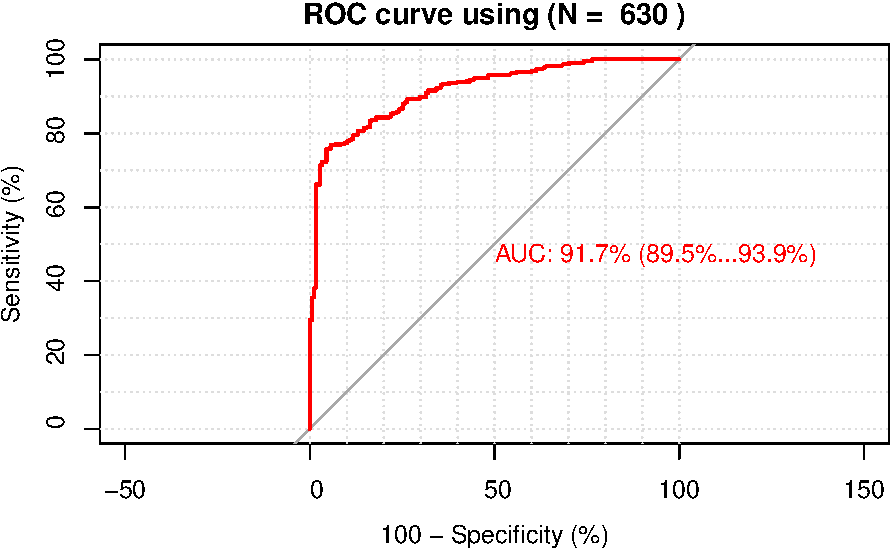
\includegraphics{AdvECTS_files/figure-latex/fishing3-1.pdf}

\begin{verbatim}
## 
## Call:
## roc.default(response = data.reduced$y, predictor = predict_model,     percent = T, ci = TRUE, plot = TRUE, boot.n = 1000, ci.alpha = 0.9,     stratified = T, grid = TRUE, show.thres = TRUE, legacy.axes = TRUE,     reuse.auc = TRUE, print.auc = TRUE, print.thres.col = "blue",     ci.type = "bars", print.thres.cex = 0.7, col = "red", main = paste("ROC curve using",         "(N = ", nrow(data.reduced), ")"))
## 
## Data: predict_model in 178 controls (data.reduced$y 0) < 452 cases (data.reduced$y 1).
## Area under the curve: 91.69%
## 95% CI: 89.5%-93.87% (DeLong)
\end{verbatim}

\hypertarget{appendix}{%
\chapter{Appendix}\label{appendix}}

\hypertarget{statistical-tables}{%
\section{Statistical Tables}\label{statistical-tables}}

\begin{table}

\caption{\label{tab:Normal}Quantiles of the $\mathcal{N}(0,1)$ distribution. If $a$ and $b$ are respectively the row and column number; then the corresponding cell gives $\mathbb{P}(0<X\le a+b)$, where $X \sim \mathcal{N}(0,1)$.}
\centering
\begin{tabular}[t]{l|r|r|r|r|r|r|r|r|r|r}
\hline
  & 0 & 0.01 & 0.02 & 0.03 & 0.04 & 0.05 & 0.06 & 0.07 & 0.08 & 0.09\\
\hline
0 & 0.5000 & 0.6179 & 0.7257 & 0.8159 & 0.8849 & 0.9332 & 0.9641 & 0.9821 & 0.9918 & 0.9965\\
\hline
0.1 & 0.5040 & 0.6217 & 0.7291 & 0.8186 & 0.8869 & 0.9345 & 0.9649 & 0.9826 & 0.9920 & 0.9966\\
\hline
0.2 & 0.5080 & 0.6255 & 0.7324 & 0.8212 & 0.8888 & 0.9357 & 0.9656 & 0.9830 & 0.9922 & 0.9967\\
\hline
0.3 & 0.5120 & 0.6293 & 0.7357 & 0.8238 & 0.8907 & 0.9370 & 0.9664 & 0.9834 & 0.9925 & 0.9968\\
\hline
0.4 & 0.5160 & 0.6331 & 0.7389 & 0.8264 & 0.8925 & 0.9382 & 0.9671 & 0.9838 & 0.9927 & 0.9969\\
\hline
0.5 & 0.5199 & 0.6368 & 0.7422 & 0.8289 & 0.8944 & 0.9394 & 0.9678 & 0.9842 & 0.9929 & 0.9970\\
\hline
0.6 & 0.5239 & 0.6406 & 0.7454 & 0.8315 & 0.8962 & 0.9406 & 0.9686 & 0.9846 & 0.9931 & 0.9971\\
\hline
0.7 & 0.5279 & 0.6443 & 0.7486 & 0.8340 & 0.8980 & 0.9418 & 0.9693 & 0.9850 & 0.9932 & 0.9972\\
\hline
0.8 & 0.5319 & 0.6480 & 0.7517 & 0.8365 & 0.8997 & 0.9429 & 0.9699 & 0.9854 & 0.9934 & 0.9973\\
\hline
0.9 & 0.5359 & 0.6517 & 0.7549 & 0.8389 & 0.9015 & 0.9441 & 0.9706 & 0.9857 & 0.9936 & 0.9974\\
\hline
1 & 0.5398 & 0.6554 & 0.7580 & 0.8413 & 0.9032 & 0.9452 & 0.9713 & 0.9861 & 0.9938 & 0.9974\\
\hline
1.1 & 0.5438 & 0.6591 & 0.7611 & 0.8438 & 0.9049 & 0.9463 & 0.9719 & 0.9864 & 0.9940 & 0.9975\\
\hline
1.2 & 0.5478 & 0.6628 & 0.7642 & 0.8461 & 0.9066 & 0.9474 & 0.9726 & 0.9868 & 0.9941 & 0.9976\\
\hline
1.3 & 0.5517 & 0.6664 & 0.7673 & 0.8485 & 0.9082 & 0.9484 & 0.9732 & 0.9871 & 0.9943 & 0.9977\\
\hline
1.4 & 0.5557 & 0.6700 & 0.7704 & 0.8508 & 0.9099 & 0.9495 & 0.9738 & 0.9875 & 0.9945 & 0.9977\\
\hline
1.5 & 0.5596 & 0.6736 & 0.7734 & 0.8531 & 0.9115 & 0.9505 & 0.9744 & 0.9878 & 0.9946 & 0.9978\\
\hline
1.6 & 0.5636 & 0.6772 & 0.7764 & 0.8554 & 0.9131 & 0.9515 & 0.9750 & 0.9881 & 0.9948 & 0.9979\\
\hline
1.7 & 0.5675 & 0.6808 & 0.7794 & 0.8577 & 0.9147 & 0.9525 & 0.9756 & 0.9884 & 0.9949 & 0.9979\\
\hline
1.8 & 0.5714 & 0.6844 & 0.7823 & 0.8599 & 0.9162 & 0.9535 & 0.9761 & 0.9887 & 0.9951 & 0.9980\\
\hline
1.9 & 0.5753 & 0.6879 & 0.7852 & 0.8621 & 0.9177 & 0.9545 & 0.9767 & 0.9890 & 0.9952 & 0.9981\\
\hline
2 & 0.5793 & 0.6915 & 0.7881 & 0.8643 & 0.9192 & 0.9554 & 0.9772 & 0.9893 & 0.9953 & 0.9981\\
\hline
2.1 & 0.5832 & 0.6950 & 0.7910 & 0.8665 & 0.9207 & 0.9564 & 0.9778 & 0.9896 & 0.9955 & 0.9982\\
\hline
2.2 & 0.5871 & 0.6985 & 0.7939 & 0.8686 & 0.9222 & 0.9573 & 0.9783 & 0.9898 & 0.9956 & 0.9982\\
\hline
2.3 & 0.5910 & 0.7019 & 0.7967 & 0.8708 & 0.9236 & 0.9582 & 0.9788 & 0.9901 & 0.9957 & 0.9983\\
\hline
2.4 & 0.5948 & 0.7054 & 0.7995 & 0.8729 & 0.9251 & 0.9591 & 0.9793 & 0.9904 & 0.9959 & 0.9984\\
\hline
2.5 & 0.5987 & 0.7088 & 0.8023 & 0.8749 & 0.9265 & 0.9599 & 0.9798 & 0.9906 & 0.9960 & 0.9984\\
\hline
2.6 & 0.6026 & 0.7123 & 0.8051 & 0.8770 & 0.9279 & 0.9608 & 0.9803 & 0.9909 & 0.9961 & 0.9985\\
\hline
2.7 & 0.6064 & 0.7157 & 0.8078 & 0.8790 & 0.9292 & 0.9616 & 0.9808 & 0.9911 & 0.9962 & 0.9985\\
\hline
2.8 & 0.6103 & 0.7190 & 0.8106 & 0.8810 & 0.9306 & 0.9625 & 0.9812 & 0.9913 & 0.9963 & 0.9986\\
\hline
2.9 & 0.6141 & 0.7224 & 0.8133 & 0.8830 & 0.9319 & 0.9633 & 0.9817 & 0.9916 & 0.9964 & 0.9986\\
\hline
\end{tabular}
\end{table}

\begin{table}

\caption{\label{tab:Student}Quantiles of the Student-$t$ distribution. The rows correspond to different degrees of freedom ($\nu$, say); the columns correspond to different probabilities ($z$, say). The cell gives $q$ that is s.t. $\mathbb{P}(-q<X<q)=z$, with $X \sim t(\nu)$.}
\centering
\begin{tabular}[t]{l|r|r|r|r|r|r|r|r}
\hline
  & 0.05 & 0.1 & 0.75 & 0.9 & 0.95 & 0.975 & 0.99 & 0.999\\
\hline
1 & 0.079 & 0.158 & 2.414 & 6.314 & 12.706 & 25.452 & 63.657 & 636.619\\
\hline
2 & 0.071 & 0.142 & 1.604 & 2.920 & 4.303 & 6.205 & 9.925 & 31.599\\
\hline
3 & 0.068 & 0.137 & 1.423 & 2.353 & 3.182 & 4.177 & 5.841 & 12.924\\
\hline
4 & 0.067 & 0.134 & 1.344 & 2.132 & 2.776 & 3.495 & 4.604 & 8.610\\
\hline
5 & 0.066 & 0.132 & 1.301 & 2.015 & 2.571 & 3.163 & 4.032 & 6.869\\
\hline
6 & 0.065 & 0.131 & 1.273 & 1.943 & 2.447 & 2.969 & 3.707 & 5.959\\
\hline
7 & 0.065 & 0.130 & 1.254 & 1.895 & 2.365 & 2.841 & 3.499 & 5.408\\
\hline
8 & 0.065 & 0.130 & 1.240 & 1.860 & 2.306 & 2.752 & 3.355 & 5.041\\
\hline
9 & 0.064 & 0.129 & 1.230 & 1.833 & 2.262 & 2.685 & 3.250 & 4.781\\
\hline
10 & 0.064 & 0.129 & 1.221 & 1.812 & 2.228 & 2.634 & 3.169 & 4.587\\
\hline
20 & 0.063 & 0.127 & 1.185 & 1.725 & 2.086 & 2.423 & 2.845 & 3.850\\
\hline
30 & 0.063 & 0.127 & 1.173 & 1.697 & 2.042 & 2.360 & 2.750 & 3.646\\
\hline
40 & 0.063 & 0.126 & 1.167 & 1.684 & 2.021 & 2.329 & 2.704 & 3.551\\
\hline
50 & 0.063 & 0.126 & 1.164 & 1.676 & 2.009 & 2.311 & 2.678 & 3.496\\
\hline
60 & 0.063 & 0.126 & 1.162 & 1.671 & 2.000 & 2.299 & 2.660 & 3.460\\
\hline
70 & 0.063 & 0.126 & 1.160 & 1.667 & 1.994 & 2.291 & 2.648 & 3.435\\
\hline
80 & 0.063 & 0.126 & 1.159 & 1.664 & 1.990 & 2.284 & 2.639 & 3.416\\
\hline
90 & 0.063 & 0.126 & 1.158 & 1.662 & 1.987 & 2.280 & 2.632 & 3.402\\
\hline
100 & 0.063 & 0.126 & 1.157 & 1.660 & 1.984 & 2.276 & 2.626 & 3.390\\
\hline
200 & 0.063 & 0.126 & 1.154 & 1.653 & 1.972 & 2.258 & 2.601 & 3.340\\
\hline
500 & 0.063 & 0.126 & 1.152 & 1.648 & 1.965 & 2.248 & 2.586 & 3.310\\
\hline
\end{tabular}
\end{table}

\begin{table}

\caption{\label{tab:Chi2}Quantiles of the $\chi^2$ distribution. The rows correspond to different degrees of freedom; the columns correspond to different probabilities.}
\centering
\begin{tabular}[t]{l|r|r|r|r|r|r|r|r}
\hline
  & 0.05 & 0.1 & 0.75 & 0.9 & 0.95 & 0.975 & 0.99 & 0.999\\
\hline
1 & 0.004 & 0.016 & 1.323 & 2.706 & 3.841 & 5.024 & 6.635 & 10.828\\
\hline
2 & 0.103 & 0.211 & 2.773 & 4.605 & 5.991 & 7.378 & 9.210 & 13.816\\
\hline
3 & 0.352 & 0.584 & 4.108 & 6.251 & 7.815 & 9.348 & 11.345 & 16.266\\
\hline
4 & 0.711 & 1.064 & 5.385 & 7.779 & 9.488 & 11.143 & 13.277 & 18.467\\
\hline
5 & 1.145 & 1.610 & 6.626 & 9.236 & 11.070 & 12.833 & 15.086 & 20.515\\
\hline
6 & 1.635 & 2.204 & 7.841 & 10.645 & 12.592 & 14.449 & 16.812 & 22.458\\
\hline
7 & 2.167 & 2.833 & 9.037 & 12.017 & 14.067 & 16.013 & 18.475 & 24.322\\
\hline
8 & 2.733 & 3.490 & 10.219 & 13.362 & 15.507 & 17.535 & 20.090 & 26.124\\
\hline
9 & 3.325 & 4.168 & 11.389 & 14.684 & 16.919 & 19.023 & 21.666 & 27.877\\
\hline
10 & 3.940 & 4.865 & 12.549 & 15.987 & 18.307 & 20.483 & 23.209 & 29.588\\
\hline
20 & 10.851 & 12.443 & 23.828 & 28.412 & 31.410 & 34.170 & 37.566 & 45.315\\
\hline
30 & 18.493 & 20.599 & 34.800 & 40.256 & 43.773 & 46.979 & 50.892 & 59.703\\
\hline
40 & 26.509 & 29.051 & 45.616 & 51.805 & 55.758 & 59.342 & 63.691 & 73.402\\
\hline
50 & 34.764 & 37.689 & 56.334 & 63.167 & 67.505 & 71.420 & 76.154 & 86.661\\
\hline
60 & 43.188 & 46.459 & 66.981 & 74.397 & 79.082 & 83.298 & 88.379 & 99.607\\
\hline
70 & 51.739 & 55.329 & 77.577 & 85.527 & 90.531 & 95.023 & 100.425 & 112.317\\
\hline
80 & 60.391 & 64.278 & 88.130 & 96.578 & 101.879 & 106.629 & 112.329 & 124.839\\
\hline
90 & 69.126 & 73.291 & 98.650 & 107.565 & 113.145 & 118.136 & 124.116 & 137.208\\
\hline
100 & 77.929 & 82.358 & 109.141 & 118.498 & 124.342 & 129.561 & 135.807 & 149.449\\
\hline
200 & 168.279 & 174.835 & 213.102 & 226.021 & 233.994 & 241.058 & 249.445 & 267.541\\
\hline
500 & 449.147 & 459.926 & 520.950 & 540.930 & 553.127 & 563.852 & 576.493 & 603.446\\
\hline
\end{tabular}
\end{table}

\begin{table}

\caption{\label{tab:Fstat}Quantiles of the $\mathcal{F}$ distribution. The columns and rows correspond to different degrees of freedom (resp. $n_1$ and $n_2$). The different panels correspond to different probabilities ($\alpha$) The corresponding cell gives $z$ that is s.t. $\mathbb{P}(X \le z)=\alpha$, with $X \sim \mathcal{F}(n_1,n_2)$.}
\centering
\begin{tabular}[t]{l|r|r|r|r|r|r|r|r|r|r}
\hline
  & 1 & 2 & 3 & 4 & 5 & 6 & 7 & 8 & 9 & 10\\
\hline
alpha = 0.9 &  &  &  &  &  &  &  &  &  & \\
\hline
5 & 4.060 & 3.780 & 3.619 & 3.520 & 3.453 & 3.405 & 3.368 & 3.339 & 3.316 & 3.297\\
\hline
10 & 3.285 & 2.924 & 2.728 & 2.605 & 2.522 & 2.461 & 2.414 & 2.377 & 2.347 & 2.323\\
\hline
15 & 3.073 & 2.695 & 2.490 & 2.361 & 2.273 & 2.208 & 2.158 & 2.119 & 2.086 & 2.059\\
\hline
20 & 2.975 & 2.589 & 2.380 & 2.249 & 2.158 & 2.091 & 2.040 & 1.999 & 1.965 & 1.937\\
\hline
50 & 2.809 & 2.412 & 2.197 & 2.061 & 1.966 & 1.895 & 1.840 & 1.796 & 1.760 & 1.729\\
\hline
100 & 2.756 & 2.356 & 2.139 & 2.002 & 1.906 & 1.834 & 1.778 & 1.732 & 1.695 & 1.663\\
\hline
500 & 2.716 & 2.313 & 2.095 & 1.956 & 1.859 & 1.786 & 1.729 & 1.683 & 1.644 & 1.612\\
\hline
alpha = 0.95 &  &  &  &  &  &  &  &  &  & \\
\hline
5 & 6.608 & 5.786 & 5.409 & 5.192 & 5.050 & 4.950 & 4.876 & 4.818 & 4.772 & 4.735\\
\hline
10 & 4.965 & 4.103 & 3.708 & 3.478 & 3.326 & 3.217 & 3.135 & 3.072 & 3.020 & 2.978\\
\hline
15 & 4.543 & 3.682 & 3.287 & 3.056 & 2.901 & 2.790 & 2.707 & 2.641 & 2.588 & 2.544\\
\hline
20 & 4.351 & 3.493 & 3.098 & 2.866 & 2.711 & 2.599 & 2.514 & 2.447 & 2.393 & 2.348\\
\hline
50 & 4.034 & 3.183 & 2.790 & 2.557 & 2.400 & 2.286 & 2.199 & 2.130 & 2.073 & 2.026\\
\hline
100 & 3.936 & 3.087 & 2.696 & 2.463 & 2.305 & 2.191 & 2.103 & 2.032 & 1.975 & 1.927\\
\hline
500 & 3.860 & 3.014 & 2.623 & 2.390 & 2.232 & 2.117 & 2.028 & 1.957 & 1.899 & 1.850\\
\hline
alpha = 0.99 &  &  &  &  &  &  &  &  &  & \\
\hline
5 & 16.258 & 13.274 & 12.060 & 11.392 & 10.967 & 10.672 & 10.456 & 10.289 & 10.158 & 10.051\\
\hline
10 & 10.044 & 7.559 & 6.552 & 5.994 & 5.636 & 5.386 & 5.200 & 5.057 & 4.942 & 4.849\\
\hline
15 & 8.683 & 6.359 & 5.417 & 4.893 & 4.556 & 4.318 & 4.142 & 4.004 & 3.895 & 3.805\\
\hline
20 & 8.096 & 5.849 & 4.938 & 4.431 & 4.103 & 3.871 & 3.699 & 3.564 & 3.457 & 3.368\\
\hline
50 & 7.171 & 5.057 & 4.199 & 3.720 & 3.408 & 3.186 & 3.020 & 2.890 & 2.785 & 2.698\\
\hline
100 & 6.895 & 4.824 & 3.984 & 3.513 & 3.206 & 2.988 & 2.823 & 2.694 & 2.590 & 2.503\\
\hline
500 & 6.686 & 4.648 & 3.821 & 3.357 & 3.054 & 2.838 & 2.675 & 2.547 & 2.443 & 2.356\\
\hline
\end{tabular}
\end{table}

\hypertarget{statistics-defintitions-and-results}{%
\section{Statistics: defintitions and results}\label{statistics-defintitions-and-results}}

\begin{definition}[Skewness and kurtosis]
\protect\hypertarget{def:skewnesskurtosis}{}\label{def:skewnesskurtosis}

Let \(Y\) be a random variable whose fourth moment exists. The expectation of \(Y\) is denoted by \(\mu\).

\begin{itemize}
\tightlist
\item
  The \{\color{blue}skewness\} of \(Y\) is given by:
  \[
  \frac{\mathbb{E}[(Y-\mu)^3]}{\{\mathbb{E}[(Y-\mu)^2]\}^{3/2}}.
  \]
\item
  The \{\color{blue}kurtosis\} of \(Y\) is given by:
  \[
  \frac{\mathbb{E}[(Y-\mu)^4]}{\{\mathbb{E}[(Y-\mu)^2]\}^{2}}.
  \]
\end{itemize}

\end{definition}

\begin{definition}[Eigenvalues]
\protect\hypertarget{def:determinant}{}\label{def:determinant}The eigenvalues of of a matrix \(M\) are the numbers \(\lambda\) for which:
\[
|M - \lambda I| = 0,
\]
where \(| \bullet |\) is the determinant operator.
\end{definition}

\begin{proposition}[Properties of the determinant]
\protect\hypertarget{prp:determinant}{}\label{prp:determinant}

We have:

\begin{itemize}
\tightlist
\item
  \(|MN|=|M|\times|N|\).
\item
  \(|M^{-1}|=|M|^{-1}\).
\item
  If \(M\) admits the diagonal representation \(M=TDT^{-1}\), where \(D\) is a diagonal matrix whose diagonal entries are \(\{\lambda_i\}_{i=1,\dots,n}\), then:
  \[
  |M - \lambda I |=\prod_{i=1}^n (\lambda_i - \lambda).
  \]
\end{itemize}

\end{proposition}

\begin{definition}[Moore-Penrose inverse]
\protect\hypertarget{def:MoorPenrose}{}\label{def:MoorPenrose}

If \(M \in \mathbb{R}^{m \times n}\), then its Moore-Penrose pseudo inverse (exists and) is the unique matrix \(M^* \in \mathbb{R}^{n \times m}\) that satisfies:

\begin{enumerate}
\def\labelenumi{\roman{enumi}.}
\tightlist
\item
  \(M M^* M = M\)
\item
  \(M^* M M^* = M^*\)
\item
  \((M M^*)'=M M^*\)
  .iv \((M^* M)'=M^* M\).
\end{enumerate}

\end{definition}

\begin{proposition}[Properties of the Moore-Penrose inverse]
\protect\hypertarget{prp:MoorPenrose}{}\label{prp:MoorPenrose}

\begin{itemize}
\tightlist
\item
  If \(M\) is invertible then \(M^* = M^{-1}\).
\item
  The pseudo-inverse of a zero matrix is its transpose.
  *

  \item*

  The pseudo-inverse of the pseudo-inverse is the original matrix.
\end{itemize}

\end{proposition}

\begin{definition}[F distribution]
\protect\hypertarget{def:fstatistics}{}\label{def:fstatistics}Consider \(n=n_1+n_2\) i.i.d. \(\mathcal{N}(0,1)\) r.v. \(X_i\). If the r.v. \(F\) is defined by:
\[
F = \frac{\sum_{i=1}^{n_1} X_i^2}{\sum_{j=n_1+1}^{n_1+n_2} X_j^2}\frac{n_2}{n_1}
\]
then \(F \sim \mathcal{F}(n_1,n_2)\). (See Table \ref{tab:Fstat} for quantiles.)
\end{definition}

\begin{definition}[Student-t distribution]
\protect\hypertarget{def:tStudent}{}\label{def:tStudent}\(Z\) follows a Student-t (or \(t\)) distribution with \(\nu\) degrees of freedom (d.f.) if:
\[
Z = X_0 \bigg/ \sqrt{\frac{\sum_{i=1}^{\nu}X_i^2}{\nu}}, \quad X_i \sim i.i.d. \mathcal{N}(0,1).
\]
We have \(\mathbb{E}(Z)=0\), and \(\mathbb{V}ar(Z)=\frac{\nu}{\nu-2}\) if \(\nu>2\). (See Table \ref{tab:Student} for quantiles.)
\end{definition}

\begin{definition}[Chi-square distribution]
\protect\hypertarget{def:chi2}{}\label{def:chi2}\(Z\) follows a \(\chi^2\) distribution with \(\nu\) d.f. if \(Z = \sum_{i=1}^{\nu}X_i^2\) where \(X_i \sim i.i.d. \mathcal{N}(0,1)\).
We have \(\mathbb{E}(Z)=\nu\). (See Table \ref{tab:Chi2} for quantiles.)
\end{definition}

\begin{definition}[Idempotent matrix]
\protect\hypertarget{def:idempotent}{}\label{def:idempotent}Matrix \(M\) is idempotent if \(M^2=M\).

If \(M\) is a symmetric idempotent matrix, then \(M'M=M\).
\end{definition}

\begin{proposition}[Roots of an idempotent matrix]
\protect\hypertarget{prp:rootsidempotent}{}\label{prp:rootsidempotent}The eigenvalues of an idempotent matrix are either 1 or 0.
\end{proposition}

\begin{proof}
If \(\lambda\) is an eigenvalue of an idempotent matrix \(M\) then \(\exists x \ne 0\) s.t. \(Mx=\lambda x\). Hence \(M^2x=\lambda M x \Rightarrow (1-\lambda)Mx=0\). Either all element of \(Mx\) are zero, in which case \(\lambda=0\) or at least one element of \(Mx\) is nonzero, in which case \(\lambda=1\).
\end{proof}

\begin{proposition}[Idempotent matrix and chi-square distribution]
\protect\hypertarget{prp:chi2idempotent}{}\label{prp:chi2idempotent}The rank of a symmetric idempotent matrix is equal to its trace.
\end{proposition}

\begin{proof}
The result follows from Prop. \ref{prp:rootsidempotent}, combined with the fact that the rank of a symmetric matrix is equal to the number of its nonzero eigenvalues.
\end{proof}

\begin{proposition}[Constrained least squares]
\protect\hypertarget{prp:constrainedLS}{}\label{prp:constrainedLS}The solution of the following optimisation problem:
\begin{eqnarray*}
\underset{\boldsymbol\beta}{\min} && || \mathbf{y} - \mathbf{X}\boldsymbol\beta ||^2 \\
&& \mbox{subject to } \mathbf{R}\boldsymbol\beta = \mathbf{q}
\end{eqnarray*}
is given by:
\[
\boxed{\boldsymbol\beta^r = \boldsymbol\beta_0 - (\mathbf{X}'\mathbf{X})^{-1} \mathbf{R}'\{\mathbf{R}(\mathbf{X}'\mathbf{X})^{-1}\mathbf{R}'\}^{-1}(\mathbf{R}\boldsymbol\beta_0 - \mathbf{q}),}
\]
where \(\boldsymbol\beta_0=(\mathbf{X}'\mathbf{X})^{-1}\mathbf{X}'\mathbf{y}\).
\end{proposition}

\begin{proof}
See for instance \href{http://jackman.stanford.edu/classes/350B/07/ftestforWeb.pdf}{Jackman, 2007}.
\end{proof}

\begin{proposition}[Chebychev's inequality]
\protect\hypertarget{prp:chebychev}{}\label{prp:chebychev}If \(\mathbb{E}(|X|^r)\) is finite for some \(r>0\) then:
\[
\forall \varepsilon > 0, \quad \mathbb{P}(|X - c|>\varepsilon) \le \frac{\mathbb{E}[|X - c|^r]}{\varepsilon^r}.
\]
In particular, for \(r=2\):
\[
\forall \varepsilon > 0, \quad \mathbb{P}(|X - c|>\varepsilon) \le \frac{\mathbb{E}[(X - c)^2]}{\varepsilon^2}.
\]
\end{proposition}

\begin{proof}
Remark that \(\varepsilon^r \mathbb{I}_{\{|X| \ge \varepsilon\}} \le |X|^r\) and take the expectation of both sides.
\end{proof}

\begin{definition}[Convergence in probability]
\protect\hypertarget{def:convergenceproba}{}\label{def:convergenceproba}The random variable sequence \(x_n\) converges in probability to a constant \(c\) if \(\forall \varepsilon\), \(\lim_{n \rightarrow \infty} \mathbb{P}(|x_n - c|>\varepsilon) = 0\).

It is denoted as: \(\mbox{plim } x_n = c\).
\end{definition}

\begin{definition}[Convergence in the Lr norm]
\protect\hypertarget{def:convergenceLr}{}\label{def:convergenceLr}\(x_n\) converges in the \(r\)-th mean (or in the \(L^r\)-norm) towards \(x\), if \(\mathbb{E}(|x_n|^r)\) and \(\mathbb{E}(|x|^r)\) exist and if
\[
\lim_{n \rightarrow \infty} \mathbb{E}(|x_n - x|^r) = 0.
\]
It is denoted as: \(x_n \overset{L^r}{\rightarrow} c\).

For \(r=2\), this convergence is called \textbf{mean square convergence}.
\end{definition}

\begin{definition}[Almost sure convergence]
\protect\hypertarget{def:convergenceAlmost}{}\label{def:convergenceAlmost}The random variable sequence \(x_n\) converges almost surely to \(c\) if \(\mathbb{P}(\lim_{n \rightarrow \infty} x_n = c) = 1\).

It is denoted as: \(x_n \overset{a.s.}{\rightarrow} c\).
\end{definition}

\begin{definition}[Convergence in distribution]
\protect\hypertarget{def:cvgcedistri}{}\label{def:cvgcedistri}\(x_n\) is said to converge in distribution (or in law) to \(x\) if
\[
\lim_{n \rightarrow \infty} F_{x_n}(s) = F_{x}(s)
\]
for all \(s\) at which \(F_X\) --the cumulative distribution of \(X\)-- is continuous.

It is denoted as: \(x_n \overset{d}{\rightarrow} x\).
\end{definition}

\begin{proposition}[Rules for limiting distributions (Slutsky)]
\protect\hypertarget{prp:Slutsky}{}\label{prp:Slutsky}

We have:

\begin{enumerate}
\def\labelenumi{\roman{enumi}.}
\item
  \textbf{Slutsky's theorem:} If \(x_n \overset{d}{\rightarrow} x\) and \(y_n \overset{p}{\rightarrow} c\) then
  \begin{eqnarray*}
  x_n y_n &\overset{d}{\rightarrow}& x c \\
  x_n + y_n &\overset{d}{\rightarrow}& x + c \\
  x_n/y_n &\overset{d}{\rightarrow}& x / c \quad (\mbox{if }c \ne 0)
  \end{eqnarray*}
\item
  \textbf{Continuous mapping theorem:} If \(x_n \overset{d}{\rightarrow} x\) and \(g\) is a continuous function then \(g(x_n) \overset{d}{\rightarrow} g(x).\)
\end{enumerate}

\end{proposition}

\begin{proposition}[Implications of stochastic convergences]
\protect\hypertarget{prp:implicationsconv}{}\label{prp:implicationsconv}We have:
\begin{align*}
&\boxed{\overset{L^s}{\rightarrow}}& &\underset{1 \le r \le s}{\Rightarrow}& &\boxed{\overset{L^r}{\rightarrow}}&\\
&& && &\Downarrow&\\
&\boxed{\overset{a.s.}{\rightarrow}}& &\Rightarrow& &\boxed{\overset{p}{\rightarrow}}& \Rightarrow \qquad \boxed{\overset{d}{\rightarrow}}.
\end{align*}
\end{proposition}

\begin{proof}
(of the fact that \(\left(\overset{p}{\rightarrow}\right) \Rightarrow \left( \overset{d}{\rightarrow}\right)\)). Assume that \(X_n \overset{p}{\rightarrow} X\). Denoting by \(F\) and \(F_n\) the c.d.f. of \(X\) and \(X_n\), respectively:
\begin{equation}
F_n(x) = \mathbb{P}(X_n \le x,X\le x+\varepsilon) + \mathbb{P}(X_n \le x,X > x+\varepsilon) \le F(x+\varepsilon) + \mathbb{P}(|X_n - X|>\varepsilon).\label{eq:convgce1}
\end{equation}
Besides,
\[
F(x-\varepsilon) = \mathbb{P}(X \le x-\varepsilon,X_n \le x) + \mathbb{P}(X \le x-\varepsilon,X_n > x) \le F_n(x) + \mathbb{P}(|X_n - X|>\varepsilon),
\]
which implies:
\begin{equation}
F(x-\varepsilon) - \mathbb{P}(|X_n - X|>\varepsilon) \le F_n(x).\label{eq:convgce2}
\end{equation}
Eqs. \eqref{eq:convgce1} and \eqref{eq:convgce2} imply:
\[
F(x-\varepsilon) - \mathbb{P}(|X_n - X|>\varepsilon) \le F_n(x)  \le F(x+\varepsilon) + \mathbb{P}(|X_n - X|>\varepsilon).
\]
Taking limits as \(n \rightarrow \infty\) yields
\[
F(x-\varepsilon) \le \underset{n \rightarrow \infty}{\mbox{lim inf}}\; F_n(x) \le \underset{n \rightarrow \infty}{\mbox{lim sup}}\; F_n(x)  \le F(x+\varepsilon).
\]
The result is then obtained by taking limits as \(\varepsilon \rightarrow 0\) (if \(F\) is continuous at \(x\)).
\end{proof}

\begin{proposition}[Convergence in distribution to a constant]
\protect\hypertarget{prp:cvgce11}{}\label{prp:cvgce11}If \(X_n\) converges in distribution to a constant \(c\), then \(X_n\) converges in probability to \(c\).
\end{proposition}

\begin{proof}
If \(\varepsilon>0\), we have \(\mathbb{P}(X_n < c - \varepsilon) \underset{n \rightarrow \infty}{\rightarrow} 0\) i.e.~\(\mathbb{P}(X_n \ge c - \varepsilon) \underset{n \rightarrow \infty}{\rightarrow} 1\) and \(\mathbb{P}(X_n < c + \varepsilon) \underset{n \rightarrow \infty}{\rightarrow} 1\). Therefore \(\mathbb{P}(c - \varepsilon \le X_n < c + \varepsilon) \underset{n \rightarrow \infty}{\rightarrow} 1\),
which gives the result.
\end{proof}

\textbf{Example of \(plim\) but not \(L^r\) convergence}: Let \(\{x_n\}_{n \in \mathbb{N}}\) be a series of random variables defined by:
\[
x_n = n u_n,
\]
where \(u_n\) are independent random variables s.t. \(u_n \sim \mathcal{B}(1/n)\).

We have \(x_n \overset{p}{\rightarrow} 0\) but \(x_n \overset{L^r}{\nrightarrow} 0\) because \(\mathbb{E}(|X_n-0|)=\mathbb{E}(X_n)=1\).

\begin{theorem}[Cauchy criterion (non-stochastic case)]
\protect\hypertarget{thm:cauchycritstatic}{}\label{thm:cauchycritstatic}We have that \(\sum_{i=0}^{T} a_i\) converges (\(T \rightarrow \infty\)) iff, for any \(\eta > 0\), there exists an integer \(N\) such that, for all \(M\ge N\),
\[
\left|\sum_{i=N+1}^{M} a_i\right| < \eta.
\]
\end{theorem}

\begin{theorem}[Cauchy criterion (stochastic case)]
\protect\hypertarget{thm:cauchycritstochastic}{}\label{thm:cauchycritstochastic}We have that \(\sum_{i=0}^{T} \theta_i \varepsilon_{t-i}\) converges in mean square (\(T \rightarrow \infty\)) to a random variable iff, for any \(\eta > 0\), there exists an integer \(N\) such that, for all \(M\ge N\),
\[
\mathbb{E}\left[\left(\sum_{i=N+1}^{M} \theta_i \varepsilon_{t-i}\right)^2\right] < \eta.
\]
\end{theorem}

\begin{definition}[Characteristic function]
\protect\hypertarget{def:characteristic}{}\label{def:characteristic}For any real-valued random variable \(X\), the characteristic function is defined by:
\[
\phi_X: u \rightarrow \mathbb{E}[\exp(iuX)].
\]
\end{definition}

\begin{theorem}[Law of large numbers]
\protect\hypertarget{thm:LLNappendix}{}\label{thm:LLNappendix}The sample mean is a consistent estimator of the population mean.
\end{theorem}

\begin{proof}
Let's denote by \(\phi_{X_i}\) the characteristic function of a r.v. \(X_i\). If the mean of \(X_i\) is \(\mu\) then the Talyor expansion of the characteristic function is:
\[
\phi_{X_i}(u) = \mathbb{E}(\exp(iuX)) = 1 + iu\mu + o(u).
\]
The properties of the characteristic function (see Def. \ref{def:characteristic}) imply that:
\[
\phi_{\frac{1}{n}(X_1+\dots+X_n)}(u) = \prod_{i=1}^{n} \left(1 + i\frac{u}{n}\mu + o\left(\frac{u}{n}\right) \right) \rightarrow e^{iu\mu}.
\]
The facts that (a) \(e^{iu\mu}\) is the characteristic function of the constant \(\mu\) and (b) that a characteristic function uniquely characterises a distribution imply that the sample mean converges in distribution to the constant \(\mu\), which further implies that it converges in probability to \(\mu\).
\end{proof}

\begin{theorem}[Lindberg-Levy Central limit theorem, CLT]
\protect\hypertarget{thm:LindbergLevyCLT}{}\label{thm:LindbergLevyCLT}If \(x_n\) is an i.i.d. sequence of random variables with mean \(\mu\) and variance \(\sigma^2\) (\(\in ]0,+\infty[\)), then:
\[
\boxed{\sqrt{n} (\bar{x}_n - \mu) \overset{d}{\rightarrow} \mathcal{N}(0,\sigma^2), \quad \mbox{where} \quad \bar{x}_n = \frac{1}{n} \sum_{i=1}^{n} x_i.}
\]
\end{theorem}

\begin{proof}
Let us introduce the r.v. \(Y_n:= \sqrt{n}(\bar{X}_n - \mu)\). We have \(\phi_{Y_n}(u) = \left[ \mathbb{E}\left( \exp(i \frac{1}{\sqrt{n}} u (X_1 - \mu)) \right) \right]^n\). We have:
\begin{eqnarray*}
\left[ \mathbb{E}\left( \exp\left(i \frac{1}{\sqrt{n}} u (X_1 - \mu)\right) \right) \right]^n &=& \left[ \mathbb{E}\left( 1 + i \frac{1}{\sqrt{n}} u (X_1 - \mu) - \frac{1}{2n} u^2 (X_1 - \mu)^2 + o(u^2) \right) \right]^n \\
&=& \left( 1 - \frac{1}{2n}u^2\sigma^2 + o(u^2)\right)^n.
\end{eqnarray*}
Therefore \(\phi_{Y_n}(u) \underset{n \rightarrow \infty}{\rightarrow} \exp \left( - \frac{1}{2}u^2\sigma^2 \right)\), which is the characteristic function of \(\mathcal{N}(0,\sigma^2)\).
\end{proof}

\begin{proposition}[Inverse of a partitioned matrix]
\protect\hypertarget{prp:inversepartitioned}{}\label{prp:inversepartitioned}We have:
\begin{eqnarray*}
&&\left[ \begin{array}{cc} \mathbf{A}_{11} & \mathbf{A}_{12} \\ \mathbf{A}_{21} & \mathbf{A}_{22} \end{array}\right]^{-1} = \\
&&\left[ \begin{array}{cc} (\mathbf{A}_{11} - \mathbf{A}_{12}\mathbf{A}_{22}^{-1}\mathbf{A}_{21})^{-1} & - \mathbf{A}_{11}^{-1}\mathbf{A}_{12}(\mathbf{A}_{22} - \mathbf{A}_{21}\mathbf{A}_{11}^{-1}\mathbf{A}_{12})^{-1} \\
-(\mathbf{A}_{22} - \mathbf{A}_{21}\mathbf{A}_{11}^{-1}\mathbf{A}_{12})^{-1}\mathbf{A}_{21}\mathbf{A}_{11}^{-1} & (\mathbf{A}_{22} - \mathbf{A}_{21}\mathbf{A}_{11}^{-1}\mathbf{A}_{12})^{-1} \end{array} \right].
\end{eqnarray*}
\end{proposition}

\begin{proposition}
\protect\hypertarget{prp:bandsindependent}{}\label{prp:bandsindependent}If \(\mathbf{A}\) is idempotent and if \(\mathbf{x}\) is Gaussian, \(\mathbf{L}\mathbf{x}\) and \(\mathbf{x}'\mathbf{A}\mathbf{x}\) are independent if \(\mathbf{L}\mathbf{A}=\mathbf{0}\).
\end{proposition}

\begin{proof}
If \(\mathbf{L}\mathbf{A}=\mathbf{0}\), then the two Gaussian vectors \(\mathbf{L}\mathbf{x}\) and \(\mathbf{A}\mathbf{x}\) are independent. This implies the independence of any function of \(\mathbf{L}\mathbf{x}\) and any function of \(\mathbf{A}\mathbf{x}\). The results then follows from the observation that \(\mathbf{x}'\mathbf{A}\mathbf{x}=(\mathbf{A}\mathbf{x})'(\mathbf{A}\mathbf{x})\), which is a function of \(\mathbf{A}\mathbf{x}\).
\end{proof}

\begin{proposition}[Inner product of a multivariate Gaussian variable]
\protect\hypertarget{prp:waldtypeproduct}{}\label{prp:waldtypeproduct}Let \(X\) be a \(n\)-dimensional multivariate Gaussian variable: \(X \sim \mathcal{N}(0,\Sigma)\). We have:
\[
X' \Sigma^{-1}X \sim \chi^2(n).
\]
\end{proposition}

\begin{proof}
Because \(\Sigma\) is a symmetrical definite positive matrix, it admits the spectral decomposition \(PDP'\) where \(P\) is an orthogonal matrix (i.e.~\(PP'=Id\)) and D is a diagonal matrix with non-negative entries. Denoting by \(\sqrt{D^{-1}}\) the diagonal matrix whose diagonal entries are the inverse of those of \(D\), it is easily checked that the covariance matrix of \(Y:=\sqrt{D^{-1}}P'X\) is \(Id\). Therefore \(Y\) is a vector of uncorrelated Gaussian variables. The properties of Gaussian variables imply that the components of \(Y\) are then also independent. Hence \(Y'Y=\sum_i Y_i^2 \sim \chi^2(n)\).

It remains to note that \(Y'Y=X'PD^{-1}P'X=X'\mathbb{V}ar(X)^{-1}X\) to conclude.
\end{proof}

\begin{theorem}[Cauchy-Schwarz inequality]
\protect\hypertarget{thm:CauchySchwarz}{}\label{thm:CauchySchwarz}We have:
\[
|\mathbb{C}ov(X,Y)| \le \sqrt{\mathbb{V}ar(X)\mathbb{V}ar(Y)}
\]
and, if \(X \ne =\) and \(Y \ne 0\), the equality holds iff \(X\) and \(Y\) are the same up to an affine transformation.
\end{theorem}

\begin{proof}
If \(\mathbb{V}ar(X)=0\), this is trivial. If this is not the case, then let's define \(Z\) as \(Z = Y - \frac{\mathbb{C}ov(X,Y)}{\mathbb{V}ar(X)}X\). It is easily seen that \(\mathbb{C}ov(X,Z)=0\). Then, the variance of \(Y=Z+\frac{\mathbb{C}ov(X,Y)}{\mathbb{V}ar(X)}X\) is equal to the sum of the variance of \(Z\) and of the variance of \(\frac{\mathbb{C}ov(X,Y)}{\mathbb{V}ar(X)}X\), that is:
\[
\mathbb{V}ar(Y) = \mathbb{V}ar(Z) + \left(\frac{\mathbb{C}ov(X,Y)}{\mathbb{V}ar(X)}\right)^2\mathbb{V}ar(X) \ge \left(\frac{\mathbb{C}ov(X,Y)}{\mathbb{V}ar(X)}\right)^2\mathbb{V}ar(X).
\]
The equality holds iff \(\mathbb{V}ar(Z)=0\), i.e.~iff \(Y = \frac{\mathbb{C}ov(X,Y)}{\mathbb{V}ar(X)}X+cst\).
\end{proof}

\begin{definition}[Matrix derivatives]
\protect\hypertarget{def:FOD}{}\label{def:FOD}Consider a fonction \(f: \mathbb{R}^K \rightarrow \mathbb{R}\). Its first-order derivative is:
\[
\frac{\partial f}{\partial \mathbf{b}}(\mathbf{b}) =
\left[\begin{array}{c}
\frac{\partial f}{\partial b_1}(\mathbf{b})\\
\vdots\\
\frac{\partial f}{\partial b_K}(\mathbf{b})
\end{array}
\right].
\]
We use the notation:
\[
\frac{\partial f}{\partial \mathbf{b}'}(\mathbf{b}) = \left(\frac{\partial f}{\partial \mathbf{b}}(\mathbf{b})\right)'.
\]
\end{definition}

\begin{proposition}
\protect\hypertarget{prp:partial}{}\label{prp:partial}

We have:

\begin{itemize}
\tightlist
\item
  If \(f(\mathbf{b}) = A' \mathbf{b}\) where \(A\) is a \(K \times 1\) vector then \(\frac{\partial f}{\partial \mathbf{b}}(\mathbf{b}) = A\).
\item
  If \(f(\mathbf{b}) = \mathbf{b}'A\mathbf{b}\) where \(A\) is a \(K \times K\) matrix, then \(\frac{\partial f}{\partial \mathbf{b}}(\mathbf{b}) = 2A\mathbf{b}\).
\end{itemize}

\end{proposition}

\begin{definition}[Asymptotic level]
\protect\hypertarget{def:asmyptlevel}{}\label{def:asmyptlevel}An asymptotic test with critical region \(\Omega_n\) has an \{\color{blue}asymptotic level\} equal to \(\alpha\) if:
\[
\underset{\theta \in \Theta}{\mbox{sup}} \quad \underset{n \rightarrow \infty}{\mbox{lim}} \mathbb{P}_\theta (S_n \in \Omega_n) = \alpha,
\]
where \(S_n\) is the test statistic and \(\Theta\) is such that the null hypothesis \(H_0\) is equivalent to \(\theta \in \Theta\).
\end{definition}

\begin{definition}[Asymptotically consistent test]
\protect\hypertarget{def:asmyptconsisttest}{}\label{def:asmyptconsisttest}An asymptotic test with critical region \(\Omega_n\) is consistent if:
\[
\forall \theta \in \Theta^c, \quad \mathbb{P}_\theta (S_n \in \Omega_n) \rightarrow 1,
\]
where \(S_n\) is the test statistic and \(\Theta^c\) is such that the null hypothesis \(H_0\) is equivalent to \(\theta \notin \Theta^c\).
\end{definition}

\begin{definition}[Kullback discrepancy]
\protect\hypertarget{def:Kullback}{}\label{def:Kullback}Given two p.d.f. \(f\) and \(f^*\), the Kullback discrepancy is defined by:
\[
I(f,f^*) = \mathbb{E}^* \left( \log \frac{f^*(Y)}{f(Y)} \right) = \int \log \frac{f^*(y)}{f(y)} f^*(y) dy.
\]
\end{definition}

\begin{center}\rule{0.5\linewidth}{0.5pt}\end{center}

\begin{proposition}[Properties of the Kullback discrepancy]
\protect\hypertarget{prp:Kullback}{}\label{prp:Kullback}

We have:

\begin{enumerate}
\def\labelenumi{\roman{enumi}.}
\item
  \(I(f,f^*) \ge 0\)
\item
  \(I(f,f^*) = 0\) iff \(f \equiv f^*\).
\end{enumerate}

\end{proposition}

\begin{center}\rule{0.5\linewidth}{0.5pt}\end{center}

\begin{proof}
\(x \rightarrow -\log(x)\) is a convex function. Therefore \(\mathbb{E}^*(-\log f(Y)/f^*(Y)) \ge -\log \mathbb{E}^*(f(Y)/f^*(Y)) = 0\) (proves (i)). Since \(x \rightarrow -\log(x)\) is strictly convex, equality in (i) holds if and only if \(f(Y)/f^*(Y)\) is constant (proves (ii)).
\end{proof}

\hypertarget{proofs}{%
\section{Proofs}\label{proofs}}

\hypertarget{MLEproperties}{%
\subsection{Proof of Proposition \ref{prp:MLEproperties}}\label{MLEproperties}}

\begin{proof}
Assumptions (i) and (ii) (in the set of Assumptions \ref{hyp:MLEregularity}) imply that \(\boldsymbol\theta_{MLE}\) exists (\(=\mbox{argmax}_\theta (1/n)\log \mathcal{L}(\boldsymbol\theta;\mathbf{y})\)).

\((1/n)\log \mathcal{L}(\boldsymbol\theta;\mathbf{y})\) can be interpreted as the sample mean of the r.v. \(\log f(Y_i;\boldsymbol\theta)\) that are i.i.d. Therefore \((1/n)\log \mathcal{L}(\boldsymbol\theta;\mathbf{y})\) converges to \(\mathbb{E}_{\boldsymbol\theta_0}(\log f(Y;\boldsymbol\theta))\) -- which exists (Assumption iv).

Because the latter convergence is uniform (Assumption v), the solution \(\boldsymbol\theta_{MLE}\) almost surely converges to the solution to the limit problem:
\[
\mbox{argmax}_\theta \mathbb{E}_{\boldsymbol\theta_0}(\log f(Y;\boldsymbol\theta)) = \mbox{argmax}_\theta \int_{\mathcal{Y}} \log f(y;\boldsymbol\theta)f(y;\boldsymbol\theta_0) dy.
\]

Properties of the Kullback information measure (see Prop. \ref{prp:Kullback}), together with the identifiability assumption (ii) implies that the solution to the limit problem is unique and equal to \(\boldsymbol\theta_0\).

Consider a r.v. sequence \(\boldsymbol\theta\) that converges to \(\boldsymbol\theta_0\). The Taylor expansion of the score in a neighborood of \(\boldsymbol\theta_0\) yields to:
\[
\frac{\partial \log \mathcal{L}(\boldsymbol\theta;\mathbf{y})}{\partial \boldsymbol\theta} = \frac{\partial \log \mathcal{L}(\boldsymbol\theta_0;\mathbf{y})}{\partial \boldsymbol\theta} + \frac{\partial^2 \log \mathcal{L}(\boldsymbol\theta_0;\mathbf{y})}{\partial \boldsymbol\theta \partial \boldsymbol\theta'}(\boldsymbol\theta - \boldsymbol\theta_0) + o_p(\boldsymbol\theta - \boldsymbol\theta_0)
\]

\(\boldsymbol\theta_{MLE}\) converges to \(\boldsymbol\theta_0\) and satisfies the likelihood equation \(\frac{\partial \log \mathcal{L}(\boldsymbol\theta;\mathbf{y})}{\partial \boldsymbol\theta} = \mathbf{0}\). Therefore:
\[
\frac{\partial \log \mathcal{L}(\boldsymbol\theta_0;\mathbf{y})}{\partial \boldsymbol\theta} \approx - \frac{\partial^2 \log \mathcal{L}(\boldsymbol\theta_0;\mathbf{y})}{\partial \boldsymbol\theta \partial \boldsymbol\theta'}(\boldsymbol\theta_{MLE} - \boldsymbol\theta_0),
\]
or equivalently:
\[
\frac{1}{\sqrt{n}} \frac{\partial \log \mathcal{L}(\boldsymbol\theta_0;\mathbf{y})}{\partial \boldsymbol\theta} \approx
\left(- \frac{1}{n} \sum_{i=1}^n \frac{\partial^2 \log f(y_i;\boldsymbol\theta_0)}{\partial \boldsymbol\theta \partial \boldsymbol\theta'} \right)\sqrt{n}(\boldsymbol\theta_{MLE} - \boldsymbol\theta_0),
\]

By the law of large numbers, we have: \(\left(- \frac{1}{n} \sum_{i=1}^n \frac{\partial^2 \log f(y_i;\boldsymbol\theta_0)}{\partial \boldsymbol\theta \partial \boldsymbol\theta'} \right) \overset{}\rightarrow \frac{1}{n} \mathbf{I}(\boldsymbol\theta_0) = \mathcal{I}_Y(\boldsymbol\theta_0)\).

Besides, we have:
\begin{eqnarray*}
\frac{1}{\sqrt{n}} \frac{\partial \log \mathcal{L}(\boldsymbol\theta_0;\mathbf{y})}{\partial \boldsymbol\theta} &=& \sqrt{n} \left( \frac{1}{n} \sum_i \frac{\partial \log f(y_i;\boldsymbol\theta_0)}{\partial \boldsymbol\theta} \right) \\
&=& \sqrt{n} \left( \frac{1}{n} \sum_i \left\{ \frac{\partial \log f(y_i;\boldsymbol\theta_0)}{\partial \boldsymbol\theta} - \mathbb{E}_{\boldsymbol\theta_0} \frac{\partial \log f(Y_i;\boldsymbol\theta_0)}{\partial \boldsymbol\theta} \right\} \right)
\end{eqnarray*}
which converges to \(\mathcal{N}(0,\mathcal{I}_Y(\boldsymbol\theta_0))\) by the CLT.

Collecting the preceding results leads to (b). The fact that \(\boldsymbol\theta_{MLE}\) achieves the FDCR bound proves (c).
\end{proof}

\hypertarget{Walddistri}{%
\subsection{Proof of Proposition \ref{prp:Walddistri}}\label{Walddistri}}

\begin{proof}
We have \(\sqrt{n}(\hat{\boldsymbol\theta}_{n} - \boldsymbol\theta_{0}) \overset{d}{\rightarrow} \mathcal{N}(0,\mathcal{I}(\boldsymbol\theta_0)^{-1})\) (Eq. \ref(eq:normMLE)). A Taylor expansion around \(\boldsymbol\theta_0\) yields to:
\begin{equation}
\sqrt{n}(h(\hat{\boldsymbol\theta}_{n}) - h(\boldsymbol\theta_{0})) \overset{d}{\rightarrow} \mathcal{N}\left(0,\frac{\partial h(\boldsymbol\theta_{0})}{\partial \boldsymbol\theta'}\mathcal{I}(\boldsymbol\theta_0)^{-1}\frac{\partial h(\boldsymbol\theta_{0})'}{\partial \boldsymbol\theta}\right). \label{eq:XXX}
\end{equation}
Under \(H_0\), \(h(\boldsymbol\theta_{0})=0\) therefore:
\begin{equation}
\sqrt{n} h(\hat{\boldsymbol\theta}_{n}) \overset{d}{\rightarrow} \mathcal{N}\left(0,\frac{\partial h(\boldsymbol\theta_{0})}{\partial \boldsymbol\theta'}\mathcal{I}(\boldsymbol\theta_0)^{-1}\frac{\partial h(\boldsymbol\theta_{0})'}{\partial \boldsymbol\theta}\right). \label{eq:lm10}
\end{equation}
Hence
\[
\sqrt{n} \left(
\frac{\partial h(\boldsymbol\theta_{0})}{\partial \boldsymbol\theta'}\mathcal{I}(\boldsymbol\theta_0)^{-1}\frac{\partial h(\boldsymbol\theta_{0})'}{\partial \boldsymbol\theta}
\right)^{-1/2} h(\hat{\boldsymbol\theta}_{n}) \overset{d}{\rightarrow} \mathcal{N}\left(0,Id\right).
\]
Taking the quadratic form, we obtain:
\[
n h(\hat{\boldsymbol\theta}_{n})'  \left(
\frac{\partial h(\boldsymbol\theta_{0})}{\partial \boldsymbol\theta'}\mathcal{I}(\boldsymbol\theta_0)^{-1}\frac{\partial h(\boldsymbol\theta_{0})'}{\partial \boldsymbol\theta}
\right)^{-1} h(\hat{\boldsymbol\theta}_{n}) \overset{d}{\rightarrow} \chi^2(r).
\]

The fact that the test has asymptotic level \(\alpha\) directly stems from what precedes. \textbf{Consistency of the test}: Consider \(\theta_0 \in \Theta\). Because the MLE is consistent, \(h(\hat{\boldsymbol\theta}_{n})\) converges to \(h(\boldsymbol\theta_0) \ne 0\). Eq. \eqref{eq:XXX} is still valid. It implies that \(\xi^W_n\) converges to \(+\infty\) and therefore that \(\mathbb{P}_{\boldsymbol\theta}(\xi^W_n \ge \chi^2_{1-\alpha}(r)) \rightarrow 1\).
\end{proof}

\hypertarget{LMdistri}{%
\subsection{Proof of Proposition \ref{prp:LMdistri}}\label{LMdistri}}

\begin{proof}
Notations: ``\(\approx\)'' means ``equal up to a term that converges to 0 in probability''. We are under \(H_0\). \(\hat{\boldsymbol\theta}^0\) is the constrained ML estimator; \(\hat{\boldsymbol\theta}\) denotes the unconstrained one.

We combine the two Taylor expansion: \(h(\hat{\boldsymbol\theta}_n) \approx \dfrac{\partial h(\boldsymbol\theta_0)}{\partial \boldsymbol\theta'}(\hat{\boldsymbol\theta}_n - \boldsymbol\theta_0)\) and \(h(\hat{\boldsymbol\theta}_n^0) \approx \dfrac{\partial h(\boldsymbol\theta_0)}{\partial \boldsymbol\theta'}(\hat{\boldsymbol\theta}_n^0 - \boldsymbol\theta_0)\) and we use \(h(\hat{\boldsymbol\theta}_n^0)=0\) (by definition) to get:
\begin{equation}
\sqrt{n}h(\hat{\boldsymbol\theta}_n) \approx \dfrac{\partial h(\boldsymbol\theta_0)}{\partial \boldsymbol\theta'}\sqrt{n}(\hat{\boldsymbol\theta}_n - \hat{\boldsymbol\theta}^0_n). \label{eq:lm1}
\end{equation}
Besides, we have (using the definition of the information matrix):
\begin{equation}
\frac{1}{\sqrt{n}}\frac{\partial \log \mathcal{L}(\hat{\boldsymbol\theta}^0_n;\mathbf{y})}{\partial \boldsymbol\theta} \approx
\frac{1}{\sqrt{n}}\frac{\partial \log \mathcal{L}(\boldsymbol\theta_0;\mathbf{y})}{\partial \boldsymbol\theta} - \mathcal{I}(\boldsymbol\theta_0)\sqrt{n}(\hat{\boldsymbol\theta}^0_n-\boldsymbol\theta_0) \label{eq:lm29}
\end{equation}
and:
\begin{equation}
0=\frac{1}{\sqrt{n}}\frac{\partial \log \mathcal{L}(\hat{\boldsymbol\theta}_n;\mathbf{y})}{\partial \boldsymbol\theta} \approx
\frac{1}{\sqrt{n}}\frac{\partial \log \mathcal{L}(\boldsymbol\theta_0;\mathbf{y})}{\partial \boldsymbol\theta} - \mathcal{I}(\boldsymbol\theta_0)\sqrt{n}(\hat{\boldsymbol\theta}_n-\boldsymbol\theta_0).\label{eq:lm30}
\end{equation}
Taking the difference and multiplying by \(\mathcal{I}(\boldsymbol\theta_0)^{-1}\):
\begin{equation}
\sqrt{n}(\hat{\boldsymbol\theta}_n-\hat{\boldsymbol\theta}_n^0) \approx
\mathcal{I}(\boldsymbol\theta_0)^{-1}\frac{1}{\sqrt{n}}\frac{\partial \log \mathcal{L}(\hat{\boldsymbol\theta}^0_n;\mathbf{y})}{\partial \boldsymbol\theta}
\mathcal{I}(\boldsymbol\theta_0).\label{eq:lm2}
\end{equation}
Eqs. \eqref{eq:lm1} and \eqref{eq:lm2} yield to:
\begin{equation}
\sqrt{n}h(\hat{\boldsymbol\theta}_n) \approx \dfrac{\partial h(\boldsymbol\theta_0)}{\partial \boldsymbol\theta'} \mathcal{I}(\boldsymbol\theta_0)^{-1}\frac{1}{\sqrt{n}}\frac{\partial \log \mathcal{L}(\hat{\boldsymbol\theta}^0_n;\mathbf{y})}{\partial \boldsymbol\theta}.\label{eq:lm3}
\end{equation}

Recall that \(\hat{\boldsymbol\theta}^0_n\) is the MLE of \(\boldsymbol\theta_0\) under the constraint \(h(\boldsymbol\theta)=0\). The vector of Lagrange multipliers \(\hat\lambda_n\) associated to this program satisfies:
\begin{equation}
\frac{\partial \log \mathcal{L}(\hat{\boldsymbol\theta}^0_n;\mathbf{y})}{\partial \boldsymbol\theta}+ \frac{\partial h'(\hat{\boldsymbol\theta}^0_n;\mathbf{y})}{\partial \boldsymbol\theta}\hat\lambda_n = 0.\label{eq:multiplier}
\end{equation}
Substituting the latter equation in Eq. \eqref{eq:lm3} gives:
\[
\sqrt{n}h(\hat{\boldsymbol\theta}_n) \approx
- \dfrac{\partial h(\boldsymbol\theta_0)}{\partial \boldsymbol\theta'} \mathcal{I}(\boldsymbol\theta_0)^{-1}
\frac{\partial h'(\hat{\boldsymbol\theta}^0_n;\mathbf{y})}{\partial \boldsymbol\theta} \frac{\hat\lambda_n}{\sqrt{n}} \approx
- \dfrac{\partial h(\boldsymbol\theta_0)}{\partial \boldsymbol\theta'} \mathcal{I}(\boldsymbol\theta_0)^{-1}
\frac{\partial h'(\boldsymbol\theta_0;\mathbf{y})}{\partial \boldsymbol\theta} \frac{\hat\lambda_n}{\sqrt{n}}
\]
which yields:
\begin{equation}
\frac{\hat\lambda_n}{\sqrt{n}} \approx - \left(
\dfrac{\partial h(\boldsymbol\theta_0)}{\partial \boldsymbol\theta'} \mathcal{I}(\boldsymbol\theta_0)^{-1}
\frac{\partial h'(\boldsymbol\theta_0;\mathbf{y})}{\partial \boldsymbol\theta}
\right)^{-1}
\sqrt{n}h(\hat{\boldsymbol\theta}_n).\label{eq:lm20}
\end{equation}
It follows, from Eq. \eqref{eq:lm10}, that:
\[
\frac{\hat\lambda_n}{\sqrt{n}} \overset{d}{\rightarrow} \mathcal{N}\left(0,\left(
\dfrac{\partial h(\boldsymbol\theta_0)}{\partial \boldsymbol\theta'} \mathcal{I}(\boldsymbol\theta_0)^{-1}
\frac{\partial h'(\boldsymbol\theta_0;\mathbf{y})}{\partial \boldsymbol\theta}
\right)^{-1}\right).
\]
Taking the quadratic form of the last equation gives:
\[
\frac{1}{n}\hat\lambda_n' \dfrac{\partial h(\hat{\boldsymbol\theta}^0_n)}{\partial \boldsymbol\theta'} \mathcal{I}(\hat{\boldsymbol\theta}^0_n)^{-1}
\frac{\partial h'(\hat{\boldsymbol\theta}^0_n;\mathbf{y})}{\partial \boldsymbol\theta} \hat\lambda_n \overset{d}{\rightarrow} \chi^2(r).
\]
Using Eq. \eqref{eq:multiplier}, it appears that the left-hand side term of the last equation is \(\xi^{LM}\) as defined in Eq. \eqref{eq:xiLM}. Consistency: see Remark 17.3 in \citet{gourieroux_monfort_1995}.
\end{proof}

\hypertarget{equivWaldLM}{%
\subsection{Proof of Proposition \ref{prp:equivWaldLM}}\label{equivWaldLM}}

\begin{proof}
We have (using Eq. \ref(eq:multiplier)):
\[
\xi^{LM}_n = \frac{1}{n}\hat\lambda_n' \dfrac{\partial h(\hat{\boldsymbol\theta}^0_n)}{\partial \boldsymbol\theta'} \mathcal{I}(\hat{\boldsymbol\theta}^0_n)^{-1}
\frac{\partial h'(\hat{\boldsymbol\theta}^0_n;\mathbf{y})}{\partial \boldsymbol\theta} \hat\lambda_n.
\]
Since, under \(H_0\), \(\hat{\boldsymbol\theta}_n^0\approx\hat{\boldsymbol\theta}_n \approx {\boldsymbol\theta}_0\), Eq. \eqref{eq:lm20} therefore implies that:
\[
\xi^{LM} \approx n h(\hat{\boldsymbol\theta}_n)' \left(
\dfrac{\partial h(\hat{\boldsymbol\theta}_n)}{\partial \boldsymbol\theta'} \mathcal{I}(\hat{\boldsymbol\theta}_n)^{-1}
\frac{\partial h'(\hat{\boldsymbol\theta}_n;\mathbf{y})}{\partial \boldsymbol\theta}
\right)^{-1}
h(\hat{\boldsymbol\theta}_n) = \xi^{W},
\]
which gives the result.
\end{proof}

\hypertarget{equivLRLM}{%
\subsection{Proof of Proposition \ref{prp:equivLRLM}}\label{equivLRLM}}

\begin{proof}
The second-order taylor expansions of \(\log \mathcal{L}(\hat{\boldsymbol\theta}^0_n,\mathbf{y})\) and \(\log \mathcal{L}(\hat{\boldsymbol\theta}_n,\mathbf{y})\) are:
\begin{eqnarray*}
\log \mathcal{L}(\hat{\boldsymbol\theta}_n,\mathbf{y}) &\approx& \log \mathcal{L}(\boldsymbol\theta_0,\mathbf{y})
+ \frac{\partial \log \mathcal{L}(\boldsymbol\theta_0,\mathbf{y})}{\partial \boldsymbol\theta'}(\hat{\boldsymbol\theta}_n-\boldsymbol\theta_0)
- \frac{n}{2} (\hat{\boldsymbol\theta}_n-\boldsymbol\theta_0)' \mathcal{I}(\boldsymbol\theta_0) (\hat{\boldsymbol\theta}_n-\boldsymbol\theta_0)\\
\log \mathcal{L}(\hat{\boldsymbol\theta}^0_n,\mathbf{y}) &\approx& \log \mathcal{L}(\boldsymbol\theta_0,\mathbf{y})
+ \frac{\partial \log \mathcal{L}(\boldsymbol\theta_0,\mathbf{y})}{\partial \boldsymbol\theta'}(\hat{\boldsymbol\theta}^0_n-\boldsymbol\theta_0)
- \frac{n}{2} (\hat{\boldsymbol\theta}^0_n-\boldsymbol\theta_0)' \mathcal{I}(\boldsymbol\theta_0) (\hat{\boldsymbol\theta}^0_n-\boldsymbol\theta_0).
\end{eqnarray*}
Taking the difference, we obtain:
\[
\xi_n^{LR} \approx 2\frac{\partial \log \mathcal{L}(\boldsymbol\theta_0,\mathbf{y})}{\partial \boldsymbol\theta'}
(\hat{\boldsymbol\theta}_n-\hat{\boldsymbol\theta}^0_n) + n (\hat{\boldsymbol\theta}^0_n-\boldsymbol\theta_0)' \mathcal{I}(\boldsymbol\theta_0) (\hat{\boldsymbol\theta}^0_n-\boldsymbol\theta_0) - n (\hat{\boldsymbol\theta}_n-\boldsymbol\theta_0)' \mathcal{I}(\boldsymbol\theta_0) (\hat{\boldsymbol\theta}_n-\boldsymbol\theta_0).
\]
Using \(\dfrac{1}{\sqrt{n}}\frac{\partial \log \mathcal{L}(\boldsymbol\theta_0;\mathbf{y})}{\partial \boldsymbol\theta} \approx \mathcal{I}(\boldsymbol\theta_0)\sqrt{n}(\hat{\boldsymbol\theta}_n-\boldsymbol\theta_0)\) (Eq. \eqref{eq:lm30}), we have:
\[
\xi_n^{LR} \approx
2n(\hat{\boldsymbol\theta}_n-\boldsymbol\theta_0)'\mathcal{I}(\boldsymbol\theta_0)
(\hat{\boldsymbol\theta}_n-\hat{\boldsymbol\theta}^0_n)
+ n (\hat{\boldsymbol\theta}^0_n-\boldsymbol\theta_0)' \mathcal{I}(\boldsymbol\theta_0) (\hat{\boldsymbol\theta}^0_n-\boldsymbol\theta_0) - n (\hat{\boldsymbol\theta}_n-\boldsymbol\theta_0)' \mathcal{I}(\boldsymbol\theta_0) (\hat{\boldsymbol\theta}_n-\boldsymbol\theta_0).
\]
In the second of the three terms in the sum, we replace \((\hat{\boldsymbol\theta}^0_n-\boldsymbol\theta_0)\) by \((\hat{\boldsymbol\theta}^0_n-\hat{\boldsymbol\theta}_n+\hat{\boldsymbol\theta}_n-\boldsymbol\theta_0)\) and we develop the associated product. This leads to:
\begin{equation}
\xi_n^{LR} \approx n (\hat{\boldsymbol\theta}^0_n-\hat{\boldsymbol\theta}_n)' \mathcal{I}(\boldsymbol\theta_0)^{-1} (\hat{\boldsymbol\theta}^0_n-\hat{\boldsymbol\theta}_n). \label{eq:lr10}
\end{equation}
The difference between Eqs. \eqref{eq:lm29} and \eqref{eq:lm30} implies:
\[
\frac{1}{\sqrt{n}}\frac{\partial \log \mathcal{L}(\hat{\boldsymbol\theta}^0_n;\mathbf{y})}{\partial \boldsymbol\theta} \approx
\mathcal{I}(\boldsymbol\theta_0)\sqrt{n}(\hat{\boldsymbol\theta}_n-\hat{\boldsymbol\theta}^0_n),
\]
which, associated to Eq. @\ref(eq:lr10), gives:
\[
\xi_n^{LR} \approx \frac{1}{n} \frac{\partial \log \mathcal{L}(\hat{\boldsymbol\theta}^0_n;\mathbf{y})}{\partial \boldsymbol\theta'} \mathcal{I}(\boldsymbol\theta_0)^{-1} \frac{\partial \log \mathcal{L}(\hat{\boldsymbol\theta}^0_n;\mathbf{y})}{\partial \boldsymbol\theta} \approx \xi_n^{LM}.
\]
Hence \(\xi_n^{LR}\) has the same asymptotic distribution as \(\xi_n^{LM}\).

Let's show that the test is consistent. For this, note that:
\[
\frac{\log \mathcal{L}(\hat{\boldsymbol\theta},\mathbf{y}) - \log \mathcal{L}(\hat{\boldsymbol\theta}^0,\mathbf{y})}{n} = \frac{1}{n} \sum_{i=1}^n[\log f(y_i;\hat{\boldsymbol\theta}_n) - \log f(y_i;\hat{\boldsymbol\theta}_n^0)] \rightarrow \mathbb{E}_0[\log f(Y;\boldsymbol\theta_0) - \log f(Y;\boldsymbol\theta_\infty)],
\]
where \(\boldsymbol\theta_\infty\), the pseudo true value, is such that \(h(\boldsymbol\theta_\infty) \ne 0\) (by definition of \(H_1\)). From the Kullback inequality and the asymptotic identifiability of \(\boldsymbol\theta_0\), it follows that \(\mathbb{E}_0[\log f(Y;\boldsymbol\theta_0) - \log f(Y;\boldsymbol\theta_\infty)] >0\). Therefore \(\xi_n^{LR} \rightarrow + \infty\) under \(H_1\).
\end{proof}

  \bibliography{book.bib,packages.bib}

\end{document}
